% Options for packages loaded elsewhere
% Options for packages loaded elsewhere
\PassOptionsToPackage{unicode}{hyperref}
\PassOptionsToPackage{hyphens}{url}
%
\documentclass[
  ignorenonframetext,
  aspectratio=169,
]{beamer}
\newif\ifbibliography
\usepackage{pgfpages}
\setbeamertemplate{caption}[numbered]
\setbeamertemplate{caption label separator}{: }
\setbeamercolor{caption name}{fg=normal text.fg}
\beamertemplatenavigationsymbolsempty
% remove section numbering
\setbeamertemplate{part page}{
  \centering
  \begin{beamercolorbox}[sep=16pt,center]{part title}
    \usebeamerfont{part title}\insertpart\par
  \end{beamercolorbox}
}
\setbeamertemplate{section page}{
  \centering
  \begin{beamercolorbox}[sep=12pt,center]{section title}
    \usebeamerfont{section title}\insertsection\par
  \end{beamercolorbox}
}
\setbeamertemplate{subsection page}{
  \centering
  \begin{beamercolorbox}[sep=8pt,center]{subsection title}
    \usebeamerfont{subsection title}\insertsubsection\par
  \end{beamercolorbox}
}
% Prevent slide breaks in the middle of a paragraph
\widowpenalties 1 10000
\raggedbottom
\AtBeginPart{
  \frame{\partpage}
}
\AtBeginSection{
  \ifbibliography
  \else
    \frame{\sectionpage}
  \fi
}
\AtBeginSubsection{
  \frame{\subsectionpage}
}
\usepackage{iftex}
\ifPDFTeX
  \usepackage[T1]{fontenc}
  \usepackage[utf8]{inputenc}
  \usepackage{textcomp} % provide euro and other symbols
\else % if luatex or xetex
  \usepackage{unicode-math} % this also loads fontspec
  \defaultfontfeatures{Scale=MatchLowercase}
  \defaultfontfeatures[\rmfamily]{Ligatures=TeX,Scale=1}
\fi
\usepackage{lmodern}

\ifPDFTeX\else
  % xetex/luatex font selection
\fi
% Use upquote if available, for straight quotes in verbatim environments
\IfFileExists{upquote.sty}{\usepackage{upquote}}{}
\IfFileExists{microtype.sty}{% use microtype if available
  \usepackage[]{microtype}
  \UseMicrotypeSet[protrusion]{basicmath} % disable protrusion for tt fonts
}{}
\makeatletter
\@ifundefined{KOMAClassName}{% if non-KOMA class
  \IfFileExists{parskip.sty}{%
    \usepackage{parskip}
  }{% else
    \setlength{\parindent}{0pt}
    \setlength{\parskip}{6pt plus 2pt minus 1pt}}
}{% if KOMA class
  \KOMAoptions{parskip=half}}
\makeatother

\usepackage{color}
\usepackage{fancyvrb}
\newcommand{\VerbBar}{|}
\newcommand{\VERB}{\Verb[commandchars=\\\{\}]}
\DefineVerbatimEnvironment{Highlighting}{Verbatim}{commandchars=\\\{\}}
% Add ',fontsize=\small' for more characters per line
\usepackage{framed}
\definecolor{shadecolor}{RGB}{241,243,245}
\newenvironment{Shaded}{\begin{snugshade}}{\end{snugshade}}
\newcommand{\AlertTok}[1]{\textcolor[rgb]{0.68,0.00,0.00}{#1}}
\newcommand{\AnnotationTok}[1]{\textcolor[rgb]{0.37,0.37,0.37}{#1}}
\newcommand{\AttributeTok}[1]{\textcolor[rgb]{0.40,0.45,0.13}{#1}}
\newcommand{\BaseNTok}[1]{\textcolor[rgb]{0.68,0.00,0.00}{#1}}
\newcommand{\BuiltInTok}[1]{\textcolor[rgb]{0.00,0.23,0.31}{#1}}
\newcommand{\CharTok}[1]{\textcolor[rgb]{0.13,0.47,0.30}{#1}}
\newcommand{\CommentTok}[1]{\textcolor[rgb]{0.37,0.37,0.37}{#1}}
\newcommand{\CommentVarTok}[1]{\textcolor[rgb]{0.37,0.37,0.37}{\textit{#1}}}
\newcommand{\ConstantTok}[1]{\textcolor[rgb]{0.56,0.35,0.01}{#1}}
\newcommand{\ControlFlowTok}[1]{\textcolor[rgb]{0.00,0.23,0.31}{\textbf{#1}}}
\newcommand{\DataTypeTok}[1]{\textcolor[rgb]{0.68,0.00,0.00}{#1}}
\newcommand{\DecValTok}[1]{\textcolor[rgb]{0.68,0.00,0.00}{#1}}
\newcommand{\DocumentationTok}[1]{\textcolor[rgb]{0.37,0.37,0.37}{\textit{#1}}}
\newcommand{\ErrorTok}[1]{\textcolor[rgb]{0.68,0.00,0.00}{#1}}
\newcommand{\ExtensionTok}[1]{\textcolor[rgb]{0.00,0.23,0.31}{#1}}
\newcommand{\FloatTok}[1]{\textcolor[rgb]{0.68,0.00,0.00}{#1}}
\newcommand{\FunctionTok}[1]{\textcolor[rgb]{0.28,0.35,0.67}{#1}}
\newcommand{\ImportTok}[1]{\textcolor[rgb]{0.00,0.46,0.62}{#1}}
\newcommand{\InformationTok}[1]{\textcolor[rgb]{0.37,0.37,0.37}{#1}}
\newcommand{\KeywordTok}[1]{\textcolor[rgb]{0.00,0.23,0.31}{\textbf{#1}}}
\newcommand{\NormalTok}[1]{\textcolor[rgb]{0.00,0.23,0.31}{#1}}
\newcommand{\OperatorTok}[1]{\textcolor[rgb]{0.37,0.37,0.37}{#1}}
\newcommand{\OtherTok}[1]{\textcolor[rgb]{0.00,0.23,0.31}{#1}}
\newcommand{\PreprocessorTok}[1]{\textcolor[rgb]{0.68,0.00,0.00}{#1}}
\newcommand{\RegionMarkerTok}[1]{\textcolor[rgb]{0.00,0.23,0.31}{#1}}
\newcommand{\SpecialCharTok}[1]{\textcolor[rgb]{0.37,0.37,0.37}{#1}}
\newcommand{\SpecialStringTok}[1]{\textcolor[rgb]{0.13,0.47,0.30}{#1}}
\newcommand{\StringTok}[1]{\textcolor[rgb]{0.13,0.47,0.30}{#1}}
\newcommand{\VariableTok}[1]{\textcolor[rgb]{0.07,0.07,0.07}{#1}}
\newcommand{\VerbatimStringTok}[1]{\textcolor[rgb]{0.13,0.47,0.30}{#1}}
\newcommand{\WarningTok}[1]{\textcolor[rgb]{0.37,0.37,0.37}{\textit{#1}}}

\usepackage{longtable,booktabs,array}
\usepackage{calc} % for calculating minipage widths
\usepackage{caption}
% Make caption package work with longtable
\makeatletter
\def\fnum@table{\tablename~\thetable}
\makeatother
\usepackage{graphicx}
\makeatletter
\newsavebox\pandoc@box
\newcommand*\pandocbounded[1]{% scales image to fit in text height/width
  \sbox\pandoc@box{#1}%
  \Gscale@div\@tempa{\textheight}{\dimexpr\ht\pandoc@box+\dp\pandoc@box\relax}%
  \Gscale@div\@tempb{\linewidth}{\wd\pandoc@box}%
  \ifdim\@tempb\p@<\@tempa\p@\let\@tempa\@tempb\fi% select the smaller of both
  \ifdim\@tempa\p@<\p@\scalebox{\@tempa}{\usebox\pandoc@box}%
  \else\usebox{\pandoc@box}%
  \fi%
}
% Set default figure placement to htbp
\def\fps@figure{htbp}
\makeatother





\setlength{\emergencystretch}{3em} % prevent overfull lines

\providecommand{\tightlist}{%
  \setlength{\itemsep}{0pt}\setlength{\parskip}{0pt}}



 


\makeatletter
\@ifpackageloaded{caption}{}{\usepackage{caption}}
\AtBeginDocument{%
\ifdefined\contentsname
  \renewcommand*\contentsname{Table of contents}
\else
  \newcommand\contentsname{Table of contents}
\fi
\ifdefined\listfigurename
  \renewcommand*\listfigurename{List of Figures}
\else
  \newcommand\listfigurename{List of Figures}
\fi
\ifdefined\listtablename
  \renewcommand*\listtablename{List of Tables}
\else
  \newcommand\listtablename{List of Tables}
\fi
\ifdefined\figurename
  \renewcommand*\figurename{Figure}
\else
  \newcommand\figurename{Figure}
\fi
\ifdefined\tablename
  \renewcommand*\tablename{Table}
\else
  \newcommand\tablename{Table}
\fi
}
\@ifpackageloaded{float}{}{\usepackage{float}}
\floatstyle{ruled}
\@ifundefined{c@chapter}{\newfloat{codelisting}{h}{lop}}{\newfloat{codelisting}{h}{lop}[chapter]}
\floatname{codelisting}{Listing}
\newcommand*\listoflistings{\listof{codelisting}{List of Listings}}
\makeatother
\makeatletter
\makeatother
\makeatletter
\@ifpackageloaded{caption}{}{\usepackage{caption}}
\@ifpackageloaded{subcaption}{}{\usepackage{subcaption}}
\makeatother

\usepackage{bookmark}
\IfFileExists{xurl.sty}{\usepackage{xurl}}{} % add URL line breaks if available
\urlstyle{same}
\hypersetup{
  pdftitle={Análise de Componentes Principais},
  hidelinks,
  pdfcreator={LaTeX via pandoc}}



\title{Análise de Componentes Principais}
\author{}
\date{}

\begin{document}
\frame{\titlepage}


\begin{frame}{Introdução}
\phantomsection\label{introduuxe7uxe3o}
Um problema central na análise de dados multivariados é a
\textbf{redução da dimensionalidade:} é possível descrever com precisão
a informação contida nos dados mensurados em \(p\) variáveis utilizando
um conjunto \(r < p\) de novas variáveis, perdendo a menor quantidade de
informação possível?

\pause

A \textbf{análise de componentes principais} tem este objetivo: dadas
\(n\) observações de \(p\) variáveis, se analisa se é possível
representar adequadamente esta informação com um número menor de
variáveis construídas como \textbf{combinações lineares} das variáveis
originais.
\end{frame}

\begin{frame}{O Problema\ldots{}}
\phantomsection\label{o-problema}
Dado um conjunto de variáveis
\(\mathbf{x} = [X_1 \hspace{0.1cm} X_2 \hspace{0.1cm} \cdots \hspace{0.1cm} X_p]^t\),
podemos encontrar outro conjunto de variáveis
\(\mathbf{y} = [Y_1 \hspace{0.1cm} Y_2 \hspace{0.1cm} \cdots \hspace{0.1cm} Y_r]^t\),
dadas por

\[Y_i= \displaystyle{\sum_{j=1}^p a_{ij}X_j}, \,\, i = 1, \cdots, r < p\]

de tal forma que a informação contida em \(\mathbf{x}\) esteja sendo bem
representada por \(\mathbf{y}\)?
\end{frame}

\begin{frame}{Algumas questões}
\phantomsection\label{algumas-questuxf5es}
Vamos encontrar combinações lineares para representar informação.

\pause

\[🤔 \text{O que é } \textbf{informação}?\]

\pause

\textbf{Informação \(\Longrightarrow\) Variância: quanto maior a
variabilidade, maior a informação contida nos dados, maior a variância
dos dados}
\end{frame}

\begin{frame}{Algumas questões}
\phantomsection\label{algumas-questuxf5es-1}
Outra questão importante:

\pause

\[🤔 \text{O que é } \textbf{uma boa representação da informação}?\]

\pause

\textbf{Boa representação da informação \(\Longrightarrow\) tomar as
componentes de \(\mathbf{y}\) que assegurem uma variância similar à de
\(\mathbf{x}\)}
\end{frame}

\begin{frame}{Esquematicamente}
\phantomsection\label{esquematicamente}
Nestas condições, temos que buscar \textbf{combinações lineares}
\(\mathbf{y}\) das variáveis \(\mathbf{x}\) de forma que se
\emph{maximize} a \textbf{variância}

\pause

\[
\begin{array}{c @{\quad} c @{\quad} c}
\hline
\textbf{Variáveis Originais} & & \textbf{Combinações Lineares} \\
\hline
X_1 & & Y_1 \\
X_2 & & Y_2 \\
\vdots & & \vdots \\
X_r & \Longrightarrow & Y_r \\
\vdots & & \vdots \\
X_p & & Y_p \\
\hline
\end{array}
\]

\pause

\[\large \mathrm{Var}[\mathbf{y}]:\ \text{Máxima}\]
\end{frame}

\begin{frame}{Esquematicamente}
\phantomsection\label{esquematicamente-1}
Ideia básica da técnica de Análise de Componentes Principais:

\pause

\[
\begin{array}{c @{\quad} c @{\quad} c}
\hline
\textbf{Variáveis Originais} & & \textbf{Componentes Principais} \\
\hline
X_1 & \text{ACP} & \color{red}{Y_1} \\
X_2 & \Longrightarrow & \color{red}{Y_2} \\
\vdots & & \color{red}{\vdots} \\
X_p & & \color{red}{Y_r} \\
 & & \vdots \\
 & & Y_p \\
\hline
\end{array}
\]

\pause

\[\scriptsize
\text{As } r \text{ primeiras componentes resumem, por exemplo, } 80\% 
\text{ do comportamento geral das } p \text{ variáveis originais.}
\]
\end{frame}

\begin{frame}{Principais objetivos}
\phantomsection\label{principais-objetivos}
\begin{itemize}
\tightlist
\item
  Redução da dimensionalidade dos dados, projetando-os em uma dimensão
  \(r < p\);
\end{itemize}

\begin{center}
\pandocbounded{\includegraphics[keepaspectratio]{../../images/CP/red_dimens.png}}
\end{center}
\end{frame}

\begin{frame}{Principais objetivos}
\phantomsection\label{principais-objetivos-1}
\begin{itemize}
\tightlist
\item
  Obtenção de combinações interpretáveis: determinar índices e produzir
  escores com base nos resultados avaliados para as \(p\) variáveis;
\end{itemize}

\begin{center}
\pandocbounded{\includegraphics[keepaspectratio]{../../images/CP/idh.png}}
\end{center}
\end{frame}

\begin{frame}{Principais objetivos}
\phantomsection\label{principais-objetivos-2}
\begin{itemize}
\tightlist
\item
  Descrição e entendimento da estrutura de correlação entre as
  variáveis, através de algumas combinações lineares das mesmas.
\end{itemize}

\begin{center}
\pandocbounded{\includegraphics[keepaspectratio]{../../images/CP/fig_pca.png}}
\end{center}
\end{frame}

\begin{frame}{Componentes Principais: o que são?}
\phantomsection\label{componentes-principais-o-que-suxe3o}
\textbf{Algebricamente:} são combinações lineares das \(p\) variáveis
originais, \(X_1, X_2, \cdots, X_p\).

\pause

\textbf{Geometricamente:} são as coordenadas dos pontos amostrais em um
sistema de eixos obtido pela rotação do sistema de eixos original, na
direção de variabilidade máxima.

\[
\Huge
\href{https://setosa.io/ev/principal-component-analysis}{\text{🔎}}
\]
\end{frame}

\begin{frame}{Componentes Principais: alguns comentários}
\phantomsection\label{componentes-principais-alguns-comentuxe1rios}
\begin{itemize}
\tightlist
\item
  Não pressupõe normalidade dos dados, embora componentes derivadas de
  populações normais tenham interpretações úteis.
\end{itemize}

\pause

\begin{itemize}
\tightlist
\item
  Com frequência, revela relações insuspeitas. Pode permitir
  interpretações que não seriam obtidas preliminarmente.
\end{itemize}

\pause

\begin{itemize}
\tightlist
\item
  Em algumas aplicações, os componentes da ACP configuram o objetivo
  final do estudo. Em outras, servem como passo intermediário para
  realização de outras análises, como regressão, classificação,
  agrupamento, etc\ldots{}
\end{itemize}
\end{frame}

\begin{frame}{Componentes Principais: como obtê-los?}
\phantomsection\label{componentes-principais-como-obtuxea-los}
\begin{itemize}
\tightlist
\item
  Sejam
  \(X_1, \hspace{0.1cm} X_2, \hspace{0.1cm} \cdots, \hspace{0.1cm} X_p\)
  as variáveis originais
\end{itemize}

\pause

\begin{itemize}
\tightlist
\item
  A ideia é encontrar um novo conjunto de variáveis
  \(Y_1, \hspace{0.1cm} Y_2, \hspace{0.1cm} \cdots, \hspace{0.1cm} Y_p\),
  tais que:
\end{itemize}

\[\textrm{Var}[Y_1] \geqslant \textrm{Var}[Y_2] \geqslant \cdots \geqslant \textrm{Var}[Y_p]\]

\pause

\begin{itemize}
\tightlist
\item
  Vamos tomar cada nova variável \(Y_i\), \(i = 1, \cdots, p\), como uma
  combinação linear das variáveis originais \(\mathbf{x}\):
\end{itemize}

\[Y_i = a_{i1}X_1 + a_{i2}X_2 + \cdots + a_{ip}X_p = \mathbf{a}_i^t \mathbf{x}\]
\end{frame}

\begin{frame}{Componentes Principais: como obtê-los?}
\phantomsection\label{componentes-principais-como-obtuxea-los-1}
\begin{itemize}
\tightlist
\item
  Para fixar problemas de escala, adicionamos uma primeira restrição aos
  vetores \(\mathbf{a}_i\):
\end{itemize}

\[\mathbf{a}_i^t \mathbf{a}_i = \displaystyle{ \sum_{j=1}^p a_{ij}^2} = 1\]

\pause

\begin{itemize}
\tightlist
\item
  Para evitar que duas variáveis \(Y_i\) e \(Y_k\), \(i \neq k\),
  \(i,k = 1, \cdots, p\), compartilhem informação, adicionamos uma
  segunda restrição aos vetores \(\mathbf{a}_i\):
\end{itemize}

\[\mathbf{a}_i^t \mathbf{a}_k = \displaystyle{ \sum_{j=1}^p a_{ij}a_{kj}}  = 0\]

\pause

\[
\textbf{💡 Garantia: } 
\quad 
\text{ortogonalidade, componentes não correlacionadas, independência}
\]
\end{frame}

\begin{frame}{Componentes Principais: como obtê-los?}
\phantomsection\label{componentes-principais-como-obtuxea-los-2}
\[
{\color{red}{\Large \textbf{Primeira Componente Principal}}}
\]

\[Y_1 = a_{11}X_1 + a_{12}X_2 + \cdots + a_{1p}X_p = \boldsymbol{a}_1^t \mathbf{x}\]

\pause

\textbf{Objetivo:} Encontrar
\(\boldsymbol{a}_1^t = [a_{11} \hspace{0.3cm} a_{12} \hspace{0.3cm} \cdots \hspace{0.3cm} a_{1p}]^t\)
tal que:

\[
{\color{red}{ \rm{Var}[Y_1]\ \text{seja máxima}}}
\]

\pause

Sujeita à restrição:

\[\boldsymbol{a}_1^t \boldsymbol{a}_1 = a_{11}^2 + a_{12}^2 + \cdots + a_{1p}^2 = 1\]
\end{frame}

\begin{frame}{Componentes Principais: como obtê-los?}
\phantomsection\label{componentes-principais-como-obtuxea-los-3}
\[
{\color{red}{\Large \textbf{Segunda Componente Principal}}}
\]

\[Y_2 = a_{21}X_1 + a_{22}X_2 + \cdots + a_{2p}X_p = \boldsymbol{a}_2^t \mathbf{x}\]

\pause

\textbf{Objetivo:} Encontrar
\(\boldsymbol{a}_2^t = [a_{21} \hspace{0.3cm} a_{22} \hspace{0.3cm} \cdots \hspace{0.3cm} a_{2p}]^t\)
tal que:

\[
{\color{red}{ \rm{Var}[Y_2]\ \text{seja máxima}}}
\]

\pause

Sujeita à restrição:

\[\boldsymbol{a}_2^t \boldsymbol{a}_2 = a_{21}^2 + a_{22}^2 + \cdots + a_{2p}^2 = 1\]

\[\rm{Cov}[Y_1,Y_2] = 0\]
\end{frame}

\begin{frame}{Componentes Principais: como obtê-los?}
\phantomsection\label{componentes-principais-como-obtuxea-los-4}
\[
{\color{red}{\Large \textbf{i-ésima Componente Principal}}}
\]

\[Y_i = a_{i1}X_1 + a_{i2}X_2 + \cdots + a_{ip}X_p = \boldsymbol{a}_i^t \mathbf{x}\]

\pause

\textbf{Objetivo:} Encontrar
\(\boldsymbol{a}_i^t = [a_{i1} \hspace{0.3cm} a_{i2} \hspace{0.3cm} \cdots \hspace{0.3cm} a_{ip}]^t\)
tal que:

\[
{\color{red}{ \rm{Var}[Y_i]\ \text{seja máxima}}}
\]

\pause

Sujeita à restrição:

\[\boldsymbol{a}_i^t \boldsymbol{a}_i =  a_{i1}^2 + a_{i2}^2 + \cdots + a_{ip}^2 = 1\]

\[\rm{Cov}[Y_,Y_k] = 0, \text{para  } k < i\]
\end{frame}

\begin{frame}{A escolha dos vetores \(\boldsymbol{a}_i\)}
\phantomsection\label{a-escolha-dos-vetores-boldsymbola_i}
\begin{itemize}
\tightlist
\item
  Considere o vetor aleatório p-variado
  \(\mathbf{x} = [X_1 \hspace{0.3cm} X_2 \hspace{0.3cm} \cdots \hspace{0.3cm} X_p]^t\)
  com vetor de médias \(\boldsymbol{\mu}\) e matriz de covariâncias
  \(\boldsymbol{\Sigma}\), positiva definida (todos os seus autovalores
  são positivos), sendo
\end{itemize}

\[\boldsymbol{\mu} = [\mu_1 \hspace{0.3cm} \mu_2 \hspace{0.3cm} \cdots \hspace{0.3cm} \mu_p]^t \hspace{0.5cm} \textrm{e} \hspace{0.5cm}
\boldsymbol{\Sigma} = \left[ \begin{array}{cccc} \sigma_{11} & \sigma_{12} & \cdots & \sigma_{1p}
\\ \sigma_{21} & \sigma_{22} & \cdots & \sigma_{2p} 
\\ \vdots & \vdots & \ddots & \vdots
\\ \sigma_{p1} & \sigma_{p2} & \cdots & \sigma_{pp} \end{array} \right]\]

\pause

\begin{itemize}
\tightlist
\item
  Para determinação dos componentes principais, com base no que foi
  exposto, usaremos o seguinte teorema:
\end{itemize}
\end{frame}

\begin{frame}{A escolha dos vetores \(\boldsymbol{a}_i\)}
\phantomsection\label{a-escolha-dos-vetores-boldsymbola_i-1}
\textbf{Teorema - Maximização de formas quadráticas:} Seja
\(\boldsymbol{B}\) uma matriz positiva definida com autovalores
\(\lambda_1 \geqslant \lambda_2 \geqslant \cdots \geqslant \lambda_p > 0\)
e autovetores associados normalizados
\({\boldsymbol{e}_1, \boldsymbol{e}_2, \cdots, \boldsymbol{e}_p}\).
Então:

\[\max_{\mathbf{x} \neq \boldsymbol{0}} \dfrac{\mathbf{x}^t \boldsymbol{B} \mathbf{x}}{\mathbf{x}^t \mathbf{x}} =  \lambda_1, \text{ obtido quando } \mathbf{x} = \boldsymbol{e}_1;\]

\[\min_{\mathbf{x} \neq \boldsymbol{0}} \dfrac{\mathbf{x}^t \boldsymbol{B} \mathbf{x}}{\mathbf{x}^t \mathbf{x}} =  \lambda_p, \text{ obtido quando } \mathbf{x} = \boldsymbol{e}_p.\]

\pause

\begin{itemize}
\tightlist
\item
  Adicionalmente,
\end{itemize}

\[\max_{\mathbf{x} \perp \boldsymbol{e}_1, \boldsymbol{e}_1, \cdots, \boldsymbol{e}_k} \dfrac{\mathbf{x}^t \boldsymbol{B} \mathbf{x}}{\mathbf{x}^t \mathbf{x}} =  \lambda_{k+1}, \text{ obtido quando } \mathbf{x} = \boldsymbol{e}_{k+1}.\]
\end{frame}

\begin{frame}{A escolha dos vetores \(\boldsymbol{a}_i\)}
\phantomsection\label{a-escolha-dos-vetores-boldsymbola_i-2}
Assim, no contexto de componentes principais, seja
\(\mathbf{x} = [X_1 \hspace{0.3cm} X_2 \hspace{0.3cm} \cdots \hspace{0.3cm} X_p]^t\)
um vetor aleatório. Seja \(\boldsymbol{\Sigma}\) a matriz de variâncias
e covariâncias e \((\lambda_1, \boldsymbol{e}_1)\),
\((\lambda_2, \boldsymbol{e}_2)\), \ldots,
\((\lambda_p, \boldsymbol{e}_p)\) seus autovalores e autovetores, tal
que
\(\lambda_1 \geqslant \lambda_2 \geqslant \cdots \geqslant \lambda_p > 0\).
Então:

\[\max_{\boldsymbol{a} \neq \boldsymbol{0}} \dfrac{\boldsymbol{a}^t \boldsymbol{\Sigma} \boldsymbol{a}}{\boldsymbol{a}^t \boldsymbol{a}} = \max_{\boldsymbol{a} \neq \boldsymbol{0}}(\boldsymbol{a}^t \boldsymbol{\Sigma} \boldsymbol{a}) = \lambda_1, \text{ obtido quando } \boldsymbol{a} = \boldsymbol{e}_1;\]

\[\min_{\boldsymbol{a} \neq \boldsymbol{0}} \dfrac{\boldsymbol{a}^t \boldsymbol{\Sigma} \boldsymbol{a}}{\boldsymbol{a}^t \boldsymbol{a}} = \min_{\boldsymbol{a} \neq \boldsymbol{0}}(\boldsymbol{a}^t \boldsymbol{\Sigma} \boldsymbol{a}) = \lambda_p, \text{ obtido quando } \boldsymbol{a} = \boldsymbol{e}_p.\]
\end{frame}

\begin{frame}{A escolha dos vetores \(\boldsymbol{a}_i\)}
\phantomsection\label{a-escolha-dos-vetores-boldsymbola_i-3}
\begin{itemize}
\tightlist
\item
  Adicionalmente,
\end{itemize}

\[\max_{\boldsymbol{a} \perp \boldsymbol{e}_1, \boldsymbol{e}_1, \cdots, \boldsymbol{e}_k} \dfrac{\boldsymbol{a}^t \boldsymbol{\Sigma} {\boldsymbol a}}{\boldsymbol{a}^t \boldsymbol{a}} = \max_{\boldsymbol{a} \perp \boldsymbol{e}_1, \boldsymbol{e}_1, \cdots, \boldsymbol{e}_k}(\boldsymbol{a}^t \boldsymbol{\Sigma} \boldsymbol{a})= \lambda_{k+1}, \text{ obtido quando } \boldsymbol{a} = \boldsymbol{e}_{k+1}.\]
\end{frame}

\begin{frame}{A escolha dos vetores \(\boldsymbol{a}_i\)}
\phantomsection\label{a-escolha-dos-vetores-boldsymbola_i-4}
\begin{itemize}
\tightlist
\item
  Uma escolha interessante para os vetores de constantes
  \({\boldsymbol{a}_i}\), \(i = 1, \cdots, p\) são os
  \textbf{autovetores normalizados} \({\boldsymbol{e}_i}\) da matriz
  \(\boldsymbol{\Sigma}\).
\end{itemize}

\pause

\begin{itemize}
\tightlist
\item
  Dessa forma, podemos definir a \(i\)-ésima componente principal da
  matriz \(\boldsymbol{\Sigma}\), \(i = 1, \cdots, p\) como sendo
\end{itemize}

\pause

\[Y_i = {\boldsymbol{e}_i^t}\mathbf{x} =  e_{i1}X_1 + e_{i2}X_2 + \cdots + e_{ip}X_p\]
\end{frame}

\begin{frame}{Componentes Principais: propriedades}
\phantomsection\label{componentes-principais-propriedades}
\begin{itemize}
\tightlist
\item
  A esperança e a variância da componente \(Y_i\) são respectivamente
  dadas por:
\end{itemize}

\[
\begin{aligned}
E[Y_i] 
  &= E[e_{i1}X_1 + e_{i2}X_2 + \cdots + e_{ip}X_p] \\
  &= e_{i1}E[X_1] + e_{i2}E[X_2] + \cdots + e_{ip}E[X_p] \\
  &= e_{i1}\mu_1 + e_{i2}\mu_2 + \cdots + e_{ip}\mu_p \\
  &= \boldsymbol{e}_i^{\mathsf{T}}\boldsymbol{\mu}
\end{aligned}
\]

\pause

\[ \textrm{Var}[Y_i] = \textrm{Var}[{\boldsymbol{e}_i^t}\mathbf{x}] = {\boldsymbol{e}_i^t} \textrm{Var}[\mathbf{x}] {\boldsymbol{e}_i}
 =  {\boldsymbol{e}_i^t} \boldsymbol{\Sigma} {\boldsymbol{e}_i} = {\boldsymbol{e}_i^t} \lambda_i {\boldsymbol{e}_i} =   
{\boldsymbol{e}_i^t} {\boldsymbol{e}_i}\lambda_i = \lambda_i \]
\end{frame}

\begin{frame}{Na forma matricial}
\phantomsection\label{na-forma-matricial}
\begin{itemize}
\tightlist
\item
  Sejam \(\boldsymbol{O}\) a matriz dos autovetores normalizados da
  matriz \(\boldsymbol{\Sigma}\), isto é,
\end{itemize}

\[\boldsymbol{O} = \left[ \begin{array}{cccc} e_{11} & e_{21} & \cdots & e_{p1}
\\ e_{12} & e_{22} & \cdots & e_{p2}
\\ \vdots & \vdots & \ddots & \vdots
\\ e_{1p} & e_{2p} & \cdots & e_{pp} \end{array} \right] = [{\boldsymbol{e}_1} \hspace{0.5cm} {\boldsymbol{e}_2}
\hspace{0.5cm} \cdots \hspace{0.5cm} {\boldsymbol{e}_p}]\]

e \(\boldsymbol{y}\) o vetor das componentes principais. Então,
\(\boldsymbol{y} = \boldsymbol{O}^t \mathbf{x}\) e a matriz de
covariâncias de \(\boldsymbol{y}\) será:

\[\textrm{Var}[\boldsymbol{y}] = \textrm{Var}[\boldsymbol{O}^t \mathbf{x}] =  \boldsymbol{O}^t \textrm{Var}[\mathbf{x}] \boldsymbol{O} =
\boldsymbol{O}^t \boldsymbol{\Sigma} \boldsymbol{O} = \boldsymbol{\Lambda}\]
\end{frame}

\begin{frame}{Na forma matricial}
\phantomsection\label{na-forma-matricial-1}
sendo

\[\boldsymbol{\Lambda} = \left[ \begin{array}{cccc} \lambda_1 & 0 & \cdots & 0
\\ 0 & \lambda_2 & \cdots & 0
\\ \vdots & \vdots & \ddots & \vdots
\\ 0 & 0 & \cdots & \lambda_p \end{array} \right] \]

ou ainda,
\(\boldsymbol{\Sigma} = \boldsymbol{O} \boldsymbol{\Lambda} \boldsymbol{O}^t = \displaystyle \sum_{i=1}^p \lambda_i \boldsymbol{e}_i \boldsymbol{e}_i^t\),
uma vez que \(\boldsymbol{O}\) é uma matriz ortogonal tal que
\(\boldsymbol{O} \boldsymbol{O}^t = \boldsymbol{O}^t \boldsymbol{O} = \boldsymbol{I}\).
Estes resultados são conhecidos como \textbf{Teorema da decomposição
espectral}.
\end{frame}

\begin{frame}{Variabilidade explicada}
\phantomsection\label{variabilidade-explicada}
\[
\begin{array}{c @{\quad} c @{\quad} c @{\quad} c}
\hline
\textbf{Variável} & \textbf{Variância} & \textbf{Componente} & \textbf{Variância} \\
\hline
X_1 & \sigma_{11} & Y_1 & \lambda_1 \\
X_2 & \sigma_{22} & Y_2 & \lambda_2 \\
\vdots & \vdots & \vdots & \vdots \\
X_p & \sigma_{pp} & Y_p & \lambda_p \\
\text{Total} 
  & \sigma_T^2 = \displaystyle\sum_{j=1}^p \sigma_{jj} = \mathrm{tr}(\boldsymbol{\Sigma})
  & \text{Total}
  & \lambda_T = \displaystyle\sum_{j=1}^p \lambda_j = \mathrm{tr}(\boldsymbol{\Lambda}) \\
\hline
\end{array}
\]

\pause

\[\rm{tr}(\boldsymbol{\Sigma}) = \rm{tr}(\boldsymbol{O} \boldsymbol{\Lambda} \boldsymbol{O}^t) = \rm{tr}(\boldsymbol{\Lambda} \boldsymbol{O}^t \boldsymbol{O}) = \rm{tr}(\boldsymbol{\Lambda} \boldsymbol{I}) = \rm{tr}(\boldsymbol{\Lambda})\]

\pause

\[\sigma_T^2 = \lambda_T\]
\end{frame}

\begin{frame}{Variabilidade explicada}
\phantomsection\label{variabilidade-explicada-1}
\begin{itemize}
\tightlist
\item
  Pode-se então concluir que a \textbf{j-ésima componente explica}
\end{itemize}

\[\displaystyle{\frac{\textrm{Var}[Y_j]}{\textrm{Variância Total de X}}} = \displaystyle{\frac{\lambda_j}{\textrm{tr}(\boldsymbol{\Sigma})}} = 
\displaystyle{\frac{\lambda_j}{\displaystyle{\sum_{i=1}^p \lambda_i}}}\]

da variação total original, e ainda, que as \textbf{\(r\) primeiras}
componentes explicam

\[\displaystyle{\frac{ \displaystyle \sum_{j=1}^r \textrm{Var}[Y_j]}{\textrm{Variância Total de X}}} = \displaystyle{\frac{\displaystyle \sum_{j=1}^r \lambda_j}{\textrm{tr}(\boldsymbol{\Sigma})}} = 
\displaystyle{\frac{\displaystyle \sum_{j=1}^r \lambda_j}{\displaystyle{\sum_{i=1}^p \lambda_i}}}\]

da variação total.
\end{frame}

\begin{frame}{Variabilidade explicada}
\phantomsection\label{variabilidade-explicada-2}
\begin{itemize}
\tightlist
\item
  Busca-se analisar um conjunto menor de variáveis sem perder muita
  informação sobre a estrutura de variabilidade original
\end{itemize}

\pause

\begin{itemize}
\tightlist
\item
  Aproximação de \(\boldsymbol{\Sigma}\): Analisando as \(r\) primeiras
  componentes principais
\end{itemize}

\[\boldsymbol{\Sigma} \approx \displaystyle \sum_{i=1}^r \lambda_i \boldsymbol{e}_i \boldsymbol{e}_i^t\]

\pause

\begin{itemize}
\tightlist
\item
  Cada parcela da soma envolve uma matriz de dimensão \(p \times p\)
  correspondente apenas à informação da \(j\)-ésima componente principal
\end{itemize}
\end{frame}

\begin{frame}{Correlação com as variáveis originais}
\phantomsection\label{correlauxe7uxe3o-com-as-variuxe1veis-originais}
\begin{itemize}
\tightlist
\item
  Os coeficientes de correlação entre a \(j\)-ésima variável e a
  \(i\)-ésima componente principal é dada por:
\end{itemize}

\[\rho_{Y_i,X_j} = \displaystyle{\frac{e_{ij} \sqrt{\lambda_i}}{\sqrt{\sigma_{jj}}}}\]

\pause

\begin{itemize}
\tightlist
\item
  As correlações medem unicamente a importância de uma variável
  individual sem considerar a influência das demais. Não medem a
  importância de \(X_i\) na presença de outras variáveis.
\end{itemize}

\pause

\begin{itemize}
\tightlist
\item
  Os coeficientes (\textbf{cargas}) dos componentes (\(e_{ij}\)), seus
  sinais e magnitudes, permitem interpretar os componentes e avaliar a
  importância das variáveis em sua constituição.
\end{itemize}
\end{frame}

\begin{frame}{Estimação das Componentes Principais}
\phantomsection\label{estimauxe7uxe3o-das-componentes-principais}
\begin{itemize}
\tightlist
\item
  Em geral, \(\boldsymbol{\Sigma}\) é estimada por \(\boldsymbol{S}\)
\end{itemize}

\[\boldsymbol{S} = \left[ \begin{array}{cccc} s_{11} & s_{12} & \cdots & s_{1p}
\\ s_{21} & s_{22} & \cdots & s_{2p} 
\\ \vdots & \vdots & \ddots & \vdots
\\ s_{p1} & s_{p2} & \cdots & s_{pp} \end{array} \right]\]

\pause

\begin{itemize}
\tightlist
\item
  Autovalores de \(\boldsymbol{S}\):
  \(\hat{\lambda}_1, \hat{\lambda}_2, \cdots, \hat{\lambda}_p\)
\end{itemize}

\pause

\begin{itemize}
\tightlist
\item
  Autovetores de \(\boldsymbol{S}\):
  \(\hat{\boldsymbol{e}}_1, \hat{\boldsymbol{e}}_2, \cdots, \hat{\boldsymbol{e}}_p\)
\end{itemize}
\end{frame}

\begin{frame}{Estimação das Componentes Principais}
\phantomsection\label{estimauxe7uxe3o-das-componentes-principais-1}
\begin{itemize}
\tightlist
\item
  Estimação da \(j\)-ésima componente principal de \(\boldsymbol{S}\):
\end{itemize}

\[\hat{Y}_j = {\hat{\boldsymbol{e}}_j^t}\mathbf{x} =  \hat{e}_{j1}X_1 + \hat{e}_{j2}X_2 + \cdots + \hat{e}_{jp}X_p, \,\,\,\,\,\, j = 1, 2, \cdots, p\]

\pause

\begin{itemize}
\tightlist
\item
  Componentes principais amostrais - Propriedades

  \begin{itemize}
  \tightlist
  \item
    Variância: \(\text{Var}(\hat{Y}_j) = \hat{\lambda}_j\)
  \item
    Covariância entre as componentes:
    \(\text{Cov}(\hat{Y}_j, \hat{Y}_k) = 0, \,\,\, j \neq k\)
  \item
    Variância total estimada explicada pela componente:
    \[\dfrac{\text{Var}(\hat{Y}_j)}{\text{Variância total estimada de } \mathbf{x}} = \dfrac{\hat{\lambda}_j}{\text{tr}(\boldsymbol{S})} =  \dfrac{\hat{\lambda}_j}{\sum \limits_{i=1}^p \hat{\lambda}_i}\]
  \end{itemize}
\end{itemize}
\end{frame}

\begin{frame}{Estimação das Componentes Principais}
\phantomsection\label{estimauxe7uxe3o-das-componentes-principais-2}
\begin{itemize}
\tightlist
\item
  Correlação estimada entre componente e variável:
  \[r_{\hat{Y}_j,\hat{X}_k} = \displaystyle{\frac{\hat{e}_{jk} \sqrt{\hat{\lambda}_j}}{\sqrt{\sigma_{kk}}}}\]
\end{itemize}

\pause

\begin{itemize}
\tightlist
\item
  Decomposição espectral de \(\boldsymbol{S}\):
\end{itemize}

\[\boldsymbol{S} = \displaystyle \sum_{j=1}^p \hat{\lambda}_j  \hat{\boldsymbol{e}}_j  \hat{\boldsymbol{e}}_j^t\]
\end{frame}

\begin{frame}{Estimação das Componentes Principais}
\phantomsection\label{estimauxe7uxe3o-das-componentes-principais-3}
\begin{itemize}
\tightlist
\item
  Aproximação de \(\boldsymbol{S}\) pelas \(r\) primeiras componentes
\end{itemize}

\[\boldsymbol{S} \approx \displaystyle \sum_{j=1}^r \hat{\lambda}_j \hat{\boldsymbol{e}}_j  \hat{\boldsymbol{e}}_j^t\]

\pause

\begin{itemize}
\tightlist
\item
  Escores das componentes

  \begin{itemize}
  \tightlist
  \item
    Valor das componentes para cada elemento amostral
  \item
    Na prática, o uso das componentes relevantes se dá através dos
    escores
  \end{itemize}
\end{itemize}
\end{frame}

\begin{frame}{Exemplo: (Mingoti,2007)}
\phantomsection\label{exemplo-mingoti2007}
\[\small
\text{12 empresas, 3 variáveis: ganho bruto }(X_1)\text{, ganho líquido }(X_2)\text{ e patrimônio acumulado }(X_3)
\]

\[\scriptsize
\begin{array}{l @{\quad} r @{\quad} r @{\quad} r}
\hline
\textbf{Empresa} &
\textbf{Ganho bruto }(X_1) &
\textbf{Ganho líquido }(X_2) &
\textbf{Patrimônio }(X_3) \\
\hline
\mathit{E1}  & 9893  & 564  & 17689 \\
\mathit{E2}  & 8776  & 389  & 17359 \\
\mathit{E3}  & 13572 & 1103 & 18597 \\
\mathit{E4}  & 6455  & 743  & 8745 \\
\mathit{E5}  & 5129  & 203  & 14397 \\
\mathit{E6}  & 5432  & 215  & 3467 \\
\mathit{E7}  & 3807  & 385  & 4679 \\
\mathit{E8}  & 3423  & 187  & 6754 \\
\mathit{E9}  & 3708  & 127  & 2275 \\
\mathit{E10} & 3294  & 297  & 6754 \\
\mathit{E11} & 5433  & 432  & 5589 \\
\mathit{E12} & 6287  & 451  & 8972 \\
\hline
\end{array}
\]
\end{frame}

\begin{frame}[fragile]{Primeiro Exemplo: (Mingoti,2007)}
\phantomsection\label{primeiro-exemplo-mingoti2007}
\begin{Shaded}
\begin{Highlighting}[]
\NormalTok{load }\OtherTok{\textless{}{-}} \ControlFlowTok{function}\NormalTok{(pkg)\{}
\NormalTok{  new.pkg }\OtherTok{\textless{}{-}}\NormalTok{ pkg[}\SpecialCharTok{!}\NormalTok{(pkg }\SpecialCharTok{\%in\%} \FunctionTok{installed.packages}\NormalTok{()[, }\StringTok{"Package"}\NormalTok{])]}
  \ControlFlowTok{if}\NormalTok{ (}\FunctionTok{length}\NormalTok{(new.pkg))}
    \FunctionTok{install.packages}\NormalTok{(new.pkg, }\AttributeTok{dependencies =} \ConstantTok{TRUE}\NormalTok{)}
  \FunctionTok{sapply}\NormalTok{(pkg, require, }\AttributeTok{character.only =} \ConstantTok{TRUE}\NormalTok{)}
\NormalTok{\} }

\DocumentationTok{\#\# Pacotes utilizados nessa análise}

\NormalTok{packages }\OtherTok{=} \FunctionTok{c}\NormalTok{(}\StringTok{"tidyverse"}\NormalTok{, }\StringTok{"factoextra"}\NormalTok{, }\StringTok{"psych"}\NormalTok{, }\StringTok{"gridExtra"}\NormalTok{)}
\FunctionTok{load}\NormalTok{(packages)}
\end{Highlighting}
\end{Shaded}

\begin{verbatim}
 tidyverse factoextra      psych  gridExtra 
      TRUE       TRUE       TRUE       TRUE 
\end{verbatim}

\begin{Shaded}
\begin{Highlighting}[]
\NormalTok{dados }\OtherTok{\textless{}{-}} \FunctionTok{read.table}\NormalTok{(}\StringTok{"https://raw.githubusercontent.com/tiagomartin/est014/refs/heads/master/dados/empresas.txt"}\NormalTok{, }\AttributeTok{row.names =} \DecValTok{1}\NormalTok{, }\AttributeTok{header =} \ConstantTok{TRUE}\NormalTok{) }
\NormalTok{dados }\SpecialCharTok{\%\textgreater{}\%} 
  \FunctionTok{str}\NormalTok{()}
\end{Highlighting}
\end{Shaded}

\begin{verbatim}
'data.frame':   12 obs. of  3 variables:
 $ Granho_Bruto : int  9893 8776 13572 6455 5129 5432 3807 3423 3708 3294 ...
 $ Ganho_Liquido: int  564 389 1103 743 203 215 385 187 127 297 ...
 $ Patrimonio   : int  17689 17359 18597 8745 14397 3467 4679 6754 2275 6754 ...
\end{verbatim}
\end{frame}

\begin{frame}[fragile]{Primeiro Exemplo: (Mingoti,2007)}
\phantomsection\label{primeiro-exemplo-mingoti2007-1}
\begin{Shaded}
\begin{Highlighting}[]
\NormalTok{x\_barra }\OtherTok{=}\NormalTok{ dados }\SpecialCharTok{\%\textgreater{}\%} 
  \FunctionTok{colMeans}\NormalTok{()}

\NormalTok{x\_barra}
\end{Highlighting}
\end{Shaded}

\begin{verbatim}
 Granho_Bruto Ganho_Liquido    Patrimonio 
    6267.4167      424.6667     9606.4167 
\end{verbatim}

\begin{Shaded}
\begin{Highlighting}[]
\NormalTok{S }\OtherTok{=}\NormalTok{ dados }\SpecialCharTok{\%\textgreater{}\%} 
  \FunctionTok{var}\NormalTok{()}

\NormalTok{S}
\end{Highlighting}
\end{Shaded}

\begin{verbatim}
              Granho_Bruto Ganho_Liquido Patrimonio
Granho_Bruto     9550608.6     706121.06 14978232.5
Ganho_Liquido     706121.1      76269.52   933915.1
Patrimonio      14978232.5     933915.06 34408113.0
\end{verbatim}
\end{frame}

\begin{frame}[fragile]{Primeiro Exemplo: (Mingoti,2007)}
\phantomsection\label{primeiro-exemplo-mingoti2007-2}
\begin{Shaded}
\begin{Highlighting}[]
\NormalTok{dados }\SpecialCharTok{\%\textgreater{}\%} 
  \FunctionTok{boxplot}\NormalTok{() }
\end{Highlighting}
\end{Shaded}

\begin{center}

\includegraphics[width=0.7\linewidth,height=\textheight,keepaspectratio]{comp_princ_files/figure-beamer/unnamed-chunk-4-1.pdf}
\end{center}
\end{frame}

\begin{frame}[fragile]{Primeiro Exemplo: (Mingoti,2007)}
\phantomsection\label{primeiro-exemplo-mingoti2007-3}
\begin{Shaded}
\begin{Highlighting}[]
\DocumentationTok{\#\# Analise de Componentes Principais utilizando a matriz de covariancias (Nao aconselhavel, neste caso)}
\NormalTok{acp\_S }\OtherTok{=} \FunctionTok{prcomp}\NormalTok{(dados)}

\DocumentationTok{\#\# Proporcao da variacao explicada}
\FunctionTok{summary}\NormalTok{(acp\_S)}
\end{Highlighting}
\end{Shaded}

\begin{verbatim}
Importance of components:
                             PC1       PC2       PC3
Standard deviation     6440.0615 1.594e+03 145.23266
Proportion of Variance    0.9418 5.767e-02   0.00048
Cumulative Proportion     0.9418 9.995e-01   1.00000
\end{verbatim}

\begin{Shaded}
\begin{Highlighting}[]
\DocumentationTok{\#\# Loadings (cargas)}
\NormalTok{acp\_S}\SpecialCharTok{$}\NormalTok{rotation}
\end{Highlighting}
\end{Shaded}

\begin{verbatim}
                      PC1         PC2         PC3
Granho_Bruto  -0.42509725 -0.89970680 -0.09909593
Ganho_Liquido -0.02766083 -0.09651661  0.99494694
Patrimonio    -0.90472493  0.42569029  0.01614231
\end{verbatim}

\begin{Shaded}
\begin{Highlighting}[]
\DocumentationTok{\#\# Opcional: trocar sinal da primeira componente e escores}
\NormalTok{acp\_S}\SpecialCharTok{$}\NormalTok{rotation }\OtherTok{=} \SpecialCharTok{{-}}\NormalTok{acp\_S}\SpecialCharTok{$}\NormalTok{rotation}
\NormalTok{acp\_S}\SpecialCharTok{$}\NormalTok{x }\OtherTok{=} \SpecialCharTok{{-}}\NormalTok{acp\_S}\SpecialCharTok{$}\NormalTok{x}

\DocumentationTok{\#\# Loadings (cargas)}
\NormalTok{acp\_S}\SpecialCharTok{$}\NormalTok{rotation}
\end{Highlighting}
\end{Shaded}

\begin{verbatim}
                     PC1         PC2         PC3
Granho_Bruto  0.42509725  0.89970680  0.09909593
Ganho_Liquido 0.02766083  0.09651661 -0.99494694
Patrimonio    0.90472493 -0.42569029 -0.01614231
\end{verbatim}
\end{frame}

\begin{frame}{Primeiro Exemplo: (Mingoti,2007)}
\phantomsection\label{primeiro-exemplo-mingoti2007-4}
\[Y_1 = 0,425 \times \text{GB} + 0,028 \times \text{GL} + 0,905 \times \text{PA} \Longrightarrow
94,18\% \text{ da informação total de } \mathbf{x}\]

\pause

\[\Large
\color{red}{\textbf{Qual a variável mais importante para } Y_1 \textbf{?}}\]

\[\Large
\textbf{Patrimônio}\]

\begin{columns}[T]
\begin{column}{0.6\linewidth}
\begin{center}
\pandocbounded{\includegraphics[keepaspectratio]{../../images/CP/empresas_bp.png}}
\end{center}
\end{column}

\begin{column}{0.4\linewidth}
\[\Huge
\color{red}{🤔 \textbf{Será?}}\]
\end{column}
\end{columns}
\end{frame}

\begin{frame}{Componentes Principais: variáveis padronizadas}
\phantomsection\label{componentes-principais-variuxe1veis-padronizadas}
\begin{itemize}
\tightlist
\item
  Padronização do vetor aleatório \(\mathbf{x}\):
\end{itemize}

\[\boldsymbol{z} = \boldsymbol{D}^{-1}(\mathbf{x} - \boldsymbol{\mu})\]

\pause

\begin{itemize}
\tightlist
\item
  \(\boldsymbol{D}\): matriz diagonal de desvios-padrão
\end{itemize}

\pause

\begin{itemize}
\tightlist
\item
  Variável padronizada:
  \(Z_i = \dfrac{X_i - \mu_i}{\sqrt{\sigma_{ii}}}\)
\end{itemize}

\pause

\begin{itemize}
\tightlist
\item
  Matriz de covariâncias de \(\boldsymbol{z}\)
\end{itemize}

\[\text{Cov}(\boldsymbol{z}) = \boldsymbol{D}^{-1}\boldsymbol{\Sigma}  \boldsymbol{D}^{-1} = \boldsymbol{P} = \text{Cor}(\mathbf{x})\]

\pause

\begin{itemize}
\tightlist
\item
  Componentes principais de \(\boldsymbol{z}\): obtidas dos autovalores
  e autovetores de \(\boldsymbol{P}\)
\end{itemize}
\end{frame}

\begin{frame}{Componentes Principais: variáveis padronizadas}
\phantomsection\label{componentes-principais-variuxe1veis-padronizadas-1}
\begin{itemize}
\tightlist
\item
  A \(j\)-ésima componente principal da matriz \(\boldsymbol{P}\):
\end{itemize}

\[Y_j = \boldsymbol{e}_j^t \boldsymbol{z} =  \boldsymbol{e}_j^t \boldsymbol{D}^{-1}(\mathbf{x} - \boldsymbol{\mu}) = {e}_{j1}Z_1 + {e}_{j2}Z_2 + \cdots + {e}_{jp}Z_p\]

sendo \(\boldsymbol{e}_j\), o \(j\)-ésimo autovetor da matriz
\(\boldsymbol{P}\), \(j = 1, \cdots p\).

\pause

\begin{itemize}
\tightlist
\item
  Variância total de \(\boldsymbol{P}\)
\end{itemize}

\[\sum \limits_{j=1}^p \text{Var}(Y_j) = \sum \limits_{j=1}^p \text{Var}(Z_j) = p\]
\end{frame}

\begin{frame}{Componentes Principais: variáveis padronizadas}
\phantomsection\label{componentes-principais-variuxe1veis-padronizadas-2}
\begin{itemize}
\tightlist
\item
  Proporção da variância populacional padronizada devido à \(j\)-ésima
  componente
\end{itemize}

\[\dfrac{\text{Var}({Y}_j)}{\text{Variância total de } \boldsymbol{z}} = \dfrac{{\lambda}_j}{\text{tr} (\boldsymbol{P})} =  \dfrac{{\lambda}_j}{p}\]

\pause

\begin{itemize}
\tightlist
\item
  Correlação entre componente \(Y_j\) e a variável padronizada \(Z_k\):
\end{itemize}

\[\rho_{Y_j,Z_k} = e_{jk} \sqrt{\lambda_j}\]
\end{frame}

\begin{frame}{Observações}
\phantomsection\label{observauxe7uxf5es}
\begin{itemize}
\tightlist
\item
  As componentes principais \textbf{não são invariantes à mudanças de
  escala}. Os resultados são \textbf{diferentes} quando se faz a análise
  utilizando a matriz de covariâncias e a matriz de correlações.
\end{itemize}

\pause

\begin{itemize}
\tightlist
\item
  \textbf{As componentes obtidas a partir da matriz de covariâncias são
  influenciadas pelas variáveis de maior variância}. A \textbf{matriz de
  correlações}, em geral, é a melhor opção quando as \textbf{variâncias
  são muito heterogêneas}.
\end{itemize}

\pause

\begin{itemize}
\tightlist
\item
  Um valor \textbf{pequeno incomum} para o \textbf{último autovalor} da
  matriz de covariâncias (ou correlação) amostral pode indicar uma
  \textbf{dependência linear não detectada} no conjunto de dados.
\end{itemize}

\pause

\begin{itemize}
\tightlist
\item
  Valores grandes de autovalores (e correspondentes autovetores) são
  importantes em uma análise.
\end{itemize}
\end{frame}

\begin{frame}{Quantas componentes devem ser retidas?}
\phantomsection\label{quantas-componentes-devem-ser-retidas}
\begin{itemize}
\tightlist
\item
  \textbf{Critério de Kaiser:} Trata-se de uma regra prática
  (heurística) para decidir quantas componentes principais manter em uma
  PCA extraída através da matriz de correlações. Ele diz:
\end{itemize}

\begin{quote}
Retenha apenas as componentes associadas a um autovalor maior que 1.
\end{quote}

\begin{itemize}
\tightlist
\item
  \(\lambda = 1\) → a componente explica tanta variabilidade quanto 1
  variável original
\item
  \(\lambda > 1\) → explica mais variabilidade do que qualquer variável
  isolada
\item
  \(\lambda < 1\) → explica menos variabilidade do que uma única
  variável → então não ``vale a pena''
\end{itemize}
\end{frame}

\begin{frame}{Quantas componentes devem ser retidas?}
\phantomsection\label{quantas-componentes-devem-ser-retidas-1}
\begin{itemize}
\tightlist
\item
  \textbf{Média dos autovalores:} É um critério alternativo quando a PCA
  é feita sobre \textbf{matriz de covariâncias}.
\end{itemize}

\begin{quote}
Se PCA foi feita na matriz de covariâncias, retenha PCs com autovalores
maiores que a média dos autovalores.
\end{quote}

Então, se uma componente tem autovalor:

\[\lambda_k > \dfrac{\sum \limits_{j=1}^p \lambda_j}{p}\]

ela retém mais informação do que a variância média por dimensão do
espaço original.
\end{frame}

\begin{frame}{Quantas componentes devem ser retidas?}
\phantomsection\label{quantas-componentes-devem-ser-retidas-2}
\begin{itemize}
\tightlist
\item
  \textbf{Screeplot:} É um gráfico que coloca, no eixo X, o número da
  componente principal e, no eixo Y, o autovalor (ou a variância
  explicada).
\end{itemize}

\begin{quote}
O ponto onde a curva deixa de cair abruptamente e começa a
``horizontalizar'' é onde você para de manter componentes.
\end{quote}

\begin{itemize}
\tightlist
\item
  A ideia é identificar o ``cotovelo'' da curva.

  \begin{itemize}
  \tightlist
  \item
    antes do cotovelo: cada componente adiciona bastante variância
  \item
    depois do cotovelo: os autovalores ficam ``quase uma linha reta'' →
    só ruído
  \end{itemize}
\end{itemize}
\end{frame}

\begin{frame}{Quantas componentes devem ser retidas?}
\phantomsection\label{quantas-componentes-devem-ser-retidas-3}
\begin{center}

\includegraphics[width=0.7\linewidth,height=\textheight,keepaspectratio]{comp_princ_files/figure-beamer/unnamed-chunk-6-1.pdf}
\end{center}
\end{frame}

\begin{frame}{Quantas componentes devem ser retidas?}
\phantomsection\label{quantas-componentes-devem-ser-retidas-4}
\begin{itemize}
\tightlist
\item
  Reter o número de componentes principais que acumulem pelo menos certa
  porcentagem da variabilidade total dos dados, digamos 70\%.
\end{itemize}

\begin{center}
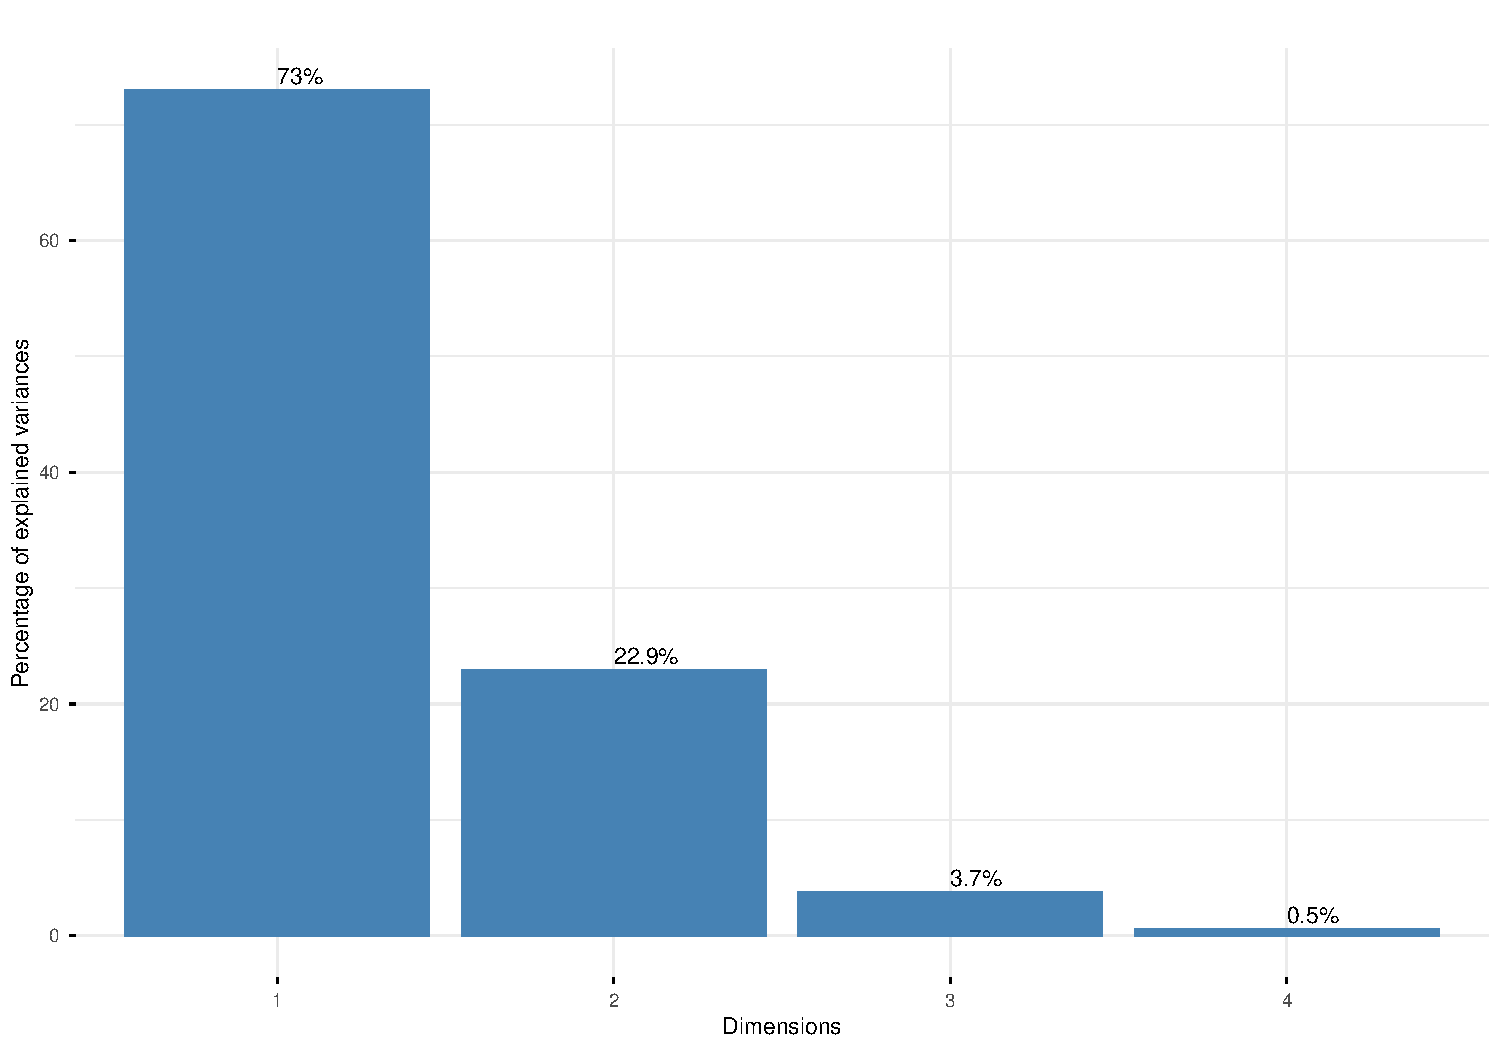
\includegraphics[width=0.7\linewidth,height=\textheight,keepaspectratio]{comp_princ_files/figure-beamer/unnamed-chunk-7-1.pdf}
\end{center}
\end{frame}

\begin{frame}{Quantas componentes devem ser retidas?}
\phantomsection\label{quantas-componentes-devem-ser-retidas-5}
\begin{itemize}
\tightlist
\item
  \textbf{Parallel Analysis (Horn, 1965):} É o método moderno mais
  recomendado para decidir quantos componentes reter em PCA.
\end{itemize}

\begin{quote}
Compare seus autovalores reais com autovalores esperados ao acaso.
\end{quote}
\end{frame}

\begin{frame}{Quantas componentes devem ser retidas?}
\phantomsection\label{quantas-componentes-devem-ser-retidas-6}
\begin{itemize}
\tightlist
\item
  O procedimento envolve:

  \begin{itemize}
  \tightlist
  \item
    Calcular os autovalores dos dados originais.
  \item
    Gerar dados aleatórios com a mesma estrutura dos dados originais.
  \item
    Calcular autovalores para os dados aleatórios, repetindo o processo
    muitas vezes para obter uma distribuição amostral.
  \item
    Comparar os autovalores reais com os autovalores médios ou percentis
    (como o 95º) dos dados simulados.
  \item
    Reter os componentes cujos autovalores reais são maiores do que os
    autovalores aleatórios correspondentes.
  \end{itemize}
\end{itemize}
\end{frame}

\begin{frame}[fragile]{Quantas componentes devem ser retidas?}
\phantomsection\label{quantas-componentes-devem-ser-retidas-7}
\begin{center}

\includegraphics[width=0.7\linewidth,height=\textheight,keepaspectratio]{comp_princ_files/figure-beamer/unnamed-chunk-8-1.pdf}
\end{center}

\begin{verbatim}
Parallel analysis suggests that the number of factors =  NA  and the number of components =  1 
\end{verbatim}
\end{frame}

\begin{frame}{Quantas componentes devem ser retidas?}
\phantomsection\label{quantas-componentes-devem-ser-retidas-8}
\begin{itemize}
\tightlist
\item
  \textbf{Interpretação desse gráfico}

  \begin{itemize}
  \tightlist
  \item
    linha azul = autovalores reais dos seus dados
  \item
    linhas vermelha / pontilhada = autovalores esperados pelo acaso
    (parallel analysis)
  \end{itemize}
\end{itemize}

\pause

\begin{itemize}
\tightlist
\item
  \textbf{Regra:} retenha apenas os componentes cuja linha azul está
  acima da linha vermelha.

  \begin{itemize}
  \tightlist
  \item
    Parallel Analysis (Horn) está dizendo: retenha 1 componente
    principal.
  \end{itemize}
\end{itemize}
\end{frame}

\begin{frame}{Interpretação das componentes principais}
\phantomsection\label{interpretauxe7uxe3o-das-componentes-principais}
\begin{itemize}
\tightlist
\item
  Em geral, quando existe uma \textbf{alta correlação positiva} entre
  todas as variáveis, os \textbf{sinais associados às variáveis
  coincidem} na primeira componente principal.
\end{itemize}

\pause

\begin{itemize}
\tightlist
\item
  Neste caso, a primeira componente principal pode ser interpretada como
  um \textbf{índice global}, calculado como uma média ponderada de todas
  as variáveis.
\end{itemize}

\pause

\begin{itemize}
\tightlist
\item
  O restante das componentes, normalmente possuem \textbf{pesos
  negativos e positivos} e são interpretadas como um \textbf{contraste
  entre grupos de variáveis}.
\end{itemize}
\end{frame}

\begin{frame}{Voltando ao Exemplo}
\phantomsection\label{voltando-ao-exemplo}
\[\small
\text{12 empresas, 3 variáveis: ganho bruto }(X_1)\text{, ganho líquido }(X_2)\text{ e patrimônio acumulado }(X_3)
\]

\[\scriptsize
\begin{array}{l @{\quad} r @{\quad} r @{\quad} r}
\hline
\textbf{Empresa} &
\textbf{Ganho bruto }(X_1) &
\textbf{Ganho líquido }(X_2) &
\textbf{Patrimônio }(X_3) \\
\hline
\mathit{E1}  & 9893  & 564  & 17689 \\
\mathit{E2}  & 8776  & 389  & 17359 \\
\mathit{E3}  & 13572 & 1103 & 18597 \\
\mathit{E4}  & 6455  & 743  & 8745 \\
\mathit{E5}  & 5129  & 203  & 14397 \\
\mathit{E6}  & 5432  & 215  & 3467 \\
\mathit{E7}  & 3807  & 385  & 4679 \\
\mathit{E8}  & 3423  & 187  & 6754 \\
\mathit{E9}  & 3708  & 127  & 2275 \\
\mathit{E10} & 3294  & 297  & 6754 \\
\mathit{E11} & 5433  & 432  & 5589 \\
\mathit{E12} & 6287  & 451  & 8972 \\
\hline
\end{array}
\]
\end{frame}

\begin{frame}{Voltando ao Exemplo}
\phantomsection\label{voltando-ao-exemplo-1}
\begin{center}
\pandocbounded{\includegraphics[keepaspectratio]{../../images/CP/empresas_bp.png}}
\end{center}
\end{frame}

\begin{frame}[fragile]{Voltando ao Exemplo}
\phantomsection\label{voltando-ao-exemplo-2}
\begin{Shaded}
\begin{Highlighting}[]
\NormalTok{dados }\SpecialCharTok{\%\textgreater{}\%} 
  \FunctionTok{scale}\NormalTok{(}\AttributeTok{center=}\ConstantTok{TRUE}\NormalTok{, }\AttributeTok{scale=}\ConstantTok{TRUE}\NormalTok{) }
\end{Highlighting}
\end{Shaded}

\begin{verbatim}
    Granho_Bruto Ganho_Liquido Patrimonio
E1   1.173173832    0.50452133  1.3779065
E2   0.811732638   -0.12914781  1.3216486
E3   2.363632341    2.45622228  1.5327010
E4   0.060698607    1.15267434 -0.1468530
E5  -0.368371244   -0.80264757  0.8166914
E6  -0.270325871   -0.75919598 -1.0466384
E7  -0.796146767   -0.14363167 -0.8400185
E8  -0.920402290   -0.86058304 -0.4862757
E9  -0.828181394   -1.07784103 -1.2498488
E10 -0.962144379   -0.46227672 -0.4862757
E11 -0.270002289    0.02655375 -0.6848831
E12  0.006336816    0.09535212 -0.1081544
attr(,"scaled:center")
 Granho_Bruto Ganho_Liquido    Patrimonio 
    6267.4167      424.6667     9606.4167 
attr(,"scaled:scale")
 Granho_Bruto Ganho_Liquido    Patrimonio 
    3090.4059      276.1694     5865.8429 
\end{verbatim}
\end{frame}

\begin{frame}[fragile]{Voltando ao Exemplo}
\phantomsection\label{voltando-ao-exemplo-3}
\begin{Shaded}
\begin{Highlighting}[]
\NormalTok{dados }\SpecialCharTok{\%\textgreater{}\%} 
  \FunctionTok{scale}\NormalTok{(}\AttributeTok{center=}\ConstantTok{TRUE}\NormalTok{, }\AttributeTok{scale=}\ConstantTok{TRUE}\NormalTok{) }\SpecialCharTok{\%\textgreater{}\%} 
  \FunctionTok{boxplot}\NormalTok{()}
\end{Highlighting}
\end{Shaded}

\begin{center}
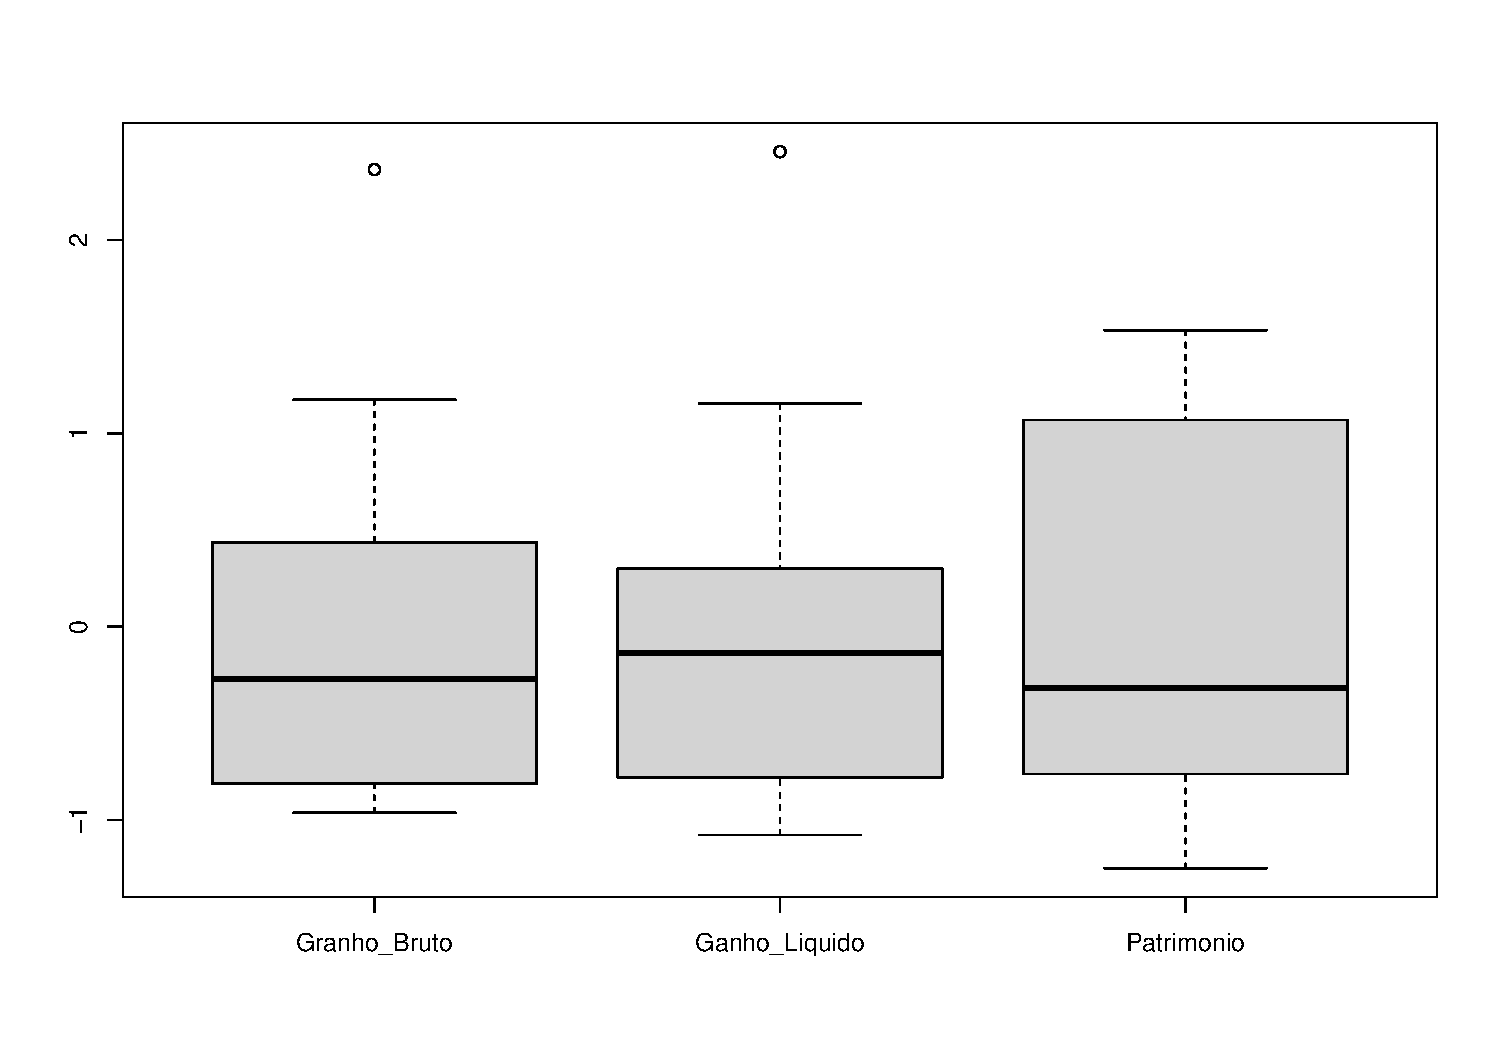
\includegraphics[width=0.7\linewidth,height=\textheight,keepaspectratio]{comp_princ_files/figure-beamer/unnamed-chunk-10-1.pdf}
\end{center}
\end{frame}

\begin{frame}[fragile]{Voltando ao Exemplo}
\phantomsection\label{voltando-ao-exemplo-4}
\begin{Shaded}
\begin{Highlighting}[]
\DocumentationTok{\#\# Analise de Componentes Principais utilizando a matriz de correlacoes (Mais aconselhavel, neste caso)}
\NormalTok{acp\_R }\OtherTok{=} \FunctionTok{prcomp}\NormalTok{(dados, }\AttributeTok{scale. =} \ConstantTok{TRUE}\NormalTok{)}

\DocumentationTok{\#\# Proporcao da variacao explicada}
\FunctionTok{summary}\NormalTok{(acp\_R)}
\end{Highlighting}
\end{Shaded}

\begin{verbatim}
Importance of components:
                          PC1    PC2     PC3
Standard deviation     1.5788 0.6508 0.28978
Proportion of Variance 0.8308 0.1412 0.02799
Cumulative Proportion  0.8308 0.9720 1.00000
\end{verbatim}

\begin{Shaded}
\begin{Highlighting}[]
\DocumentationTok{\#\# Loadings (cargas)}
\NormalTok{acp\_R}\SpecialCharTok{$}\NormalTok{rotation}
\end{Highlighting}
\end{Shaded}

\begin{verbatim}
                     PC1          PC2        PC3
Granho_Bruto  -0.6167027  0.001267206  0.7871952
Ganho_Liquido -0.5567945  0.706196936 -0.4373395
Patrimonio    -0.5564690 -0.708014324 -0.4348080
\end{verbatim}

\begin{Shaded}
\begin{Highlighting}[]
\DocumentationTok{\#\# Opcional: trocar sinal da primeira componente e escores}
\NormalTok{acp\_R}\SpecialCharTok{$}\NormalTok{rotation }\OtherTok{=} \SpecialCharTok{{-}}\NormalTok{acp\_R}\SpecialCharTok{$}\NormalTok{rotation}
\NormalTok{acp\_R}\SpecialCharTok{$}\NormalTok{x }\OtherTok{=} \SpecialCharTok{{-}}\NormalTok{acp\_R}\SpecialCharTok{$}\NormalTok{x}

\DocumentationTok{\#\# Loadings (cargas)}
\NormalTok{acp\_R}\SpecialCharTok{$}\NormalTok{rotation}
\end{Highlighting}
\end{Shaded}

\begin{verbatim}
                    PC1          PC2        PC3
Granho_Bruto  0.6167027 -0.001267206 -0.7871952
Ganho_Liquido 0.5567945 -0.706196936  0.4373395
Patrimonio    0.5564690  0.708014324  0.4348080
\end{verbatim}
\end{frame}

\begin{frame}[fragile]{Voltando ao Exemplo}
\phantomsection\label{voltando-ao-exemplo-5}
\begin{Shaded}
\begin{Highlighting}[]
\DocumentationTok{\#\# Escores das componentes principais}
\NormalTok{Yr }\OtherTok{=}\NormalTok{ acp\_R}\SpecialCharTok{$}\NormalTok{x}
\NormalTok{Yr }\SpecialCharTok{\%\textgreater{}\%} \FunctionTok{head}\NormalTok{()}
\end{Highlighting}
\end{Shaded}

\begin{verbatim}
          PC1        PC2        PC3
E1  1.7711764  0.6177995 -0.1037449
E2  1.1641454  1.0259213 -0.1208101
E3  3.6781699 -0.6523976 -0.1200063
E4  0.5975165 -0.9180660  0.3924755
E5 -0.2196218  1.1455233  0.2940545
E6 -1.1718486 -0.2045506 -0.5743139
\end{verbatim}

\begin{Shaded}
\begin{Highlighting}[]
\DocumentationTok{\#\# Matriz de correlacoes entre variaveis originais e componentes principais}
\NormalTok{Ryx\_R }\OtherTok{=} \FunctionTok{cor}\NormalTok{(dados,Yr)}
\NormalTok{Ryx\_R}
\end{Highlighting}
\end{Shaded}

\begin{verbatim}
                    PC1           PC2        PC3
Granho_Bruto  0.9736351 -0.0008246563 -0.2281098
Ganho_Liquido 0.8790534 -0.4595699002  0.1267302
Patrimonio    0.8785396  0.4607525968  0.1259966
\end{verbatim}
\end{frame}

\begin{frame}[fragile]{Voltando ao Exemplo}
\phantomsection\label{voltando-ao-exemplo-6}
\begin{Shaded}
\begin{Highlighting}[]
\FunctionTok{fa.parallel}\NormalTok{(dados }\SpecialCharTok{\%\textgreater{}\%} \FunctionTok{scale}\NormalTok{(}\AttributeTok{center=}\ConstantTok{TRUE}\NormalTok{, }\AttributeTok{scale=}\ConstantTok{TRUE}\NormalTok{), }\AttributeTok{fa=}\StringTok{"pc"}\NormalTok{, }\AttributeTok{n.iter=}\DecValTok{1000}\NormalTok{)}
\end{Highlighting}
\end{Shaded}

\begin{center}

\includegraphics[width=0.7\linewidth,height=\textheight,keepaspectratio]{comp_princ_files/figure-beamer/unnamed-chunk-14-1.pdf}
\end{center}

\begin{verbatim}
Parallel analysis suggests that the number of factors =  NA  and the number of components =  1 
\end{verbatim}
\end{frame}

\begin{frame}{Voltando ao Exemplo}
\phantomsection\label{voltando-ao-exemplo-7}
\[Z_{GB} = \dfrac{\text{Ganho Bruto} - \overline{\text{Ganho Bruto}}}{s_{\text{Ganho Bruto}}}\]

\[Z_{GL} = \dfrac{\text{Ganho Líquido} - \overline{\text{Ganho Líquido}}}{s_{\text{Ganho Líquido}}}\]

\[Z_{PA} = \dfrac{\text{Patrimônio} - \overline{\text{Patrimônio}}}{s_{\text{Patrimônio}}}\]
\end{frame}

\begin{frame}{Voltando ao Exemplo}
\phantomsection\label{voltando-ao-exemplo-8}
\[Y_1 =  0,617 \times Z_{GB} + 0,557 \times Z_{GL} + 0,556 \times Z_{PA} \Longrightarrow
83,08\% \text{ da informação total de } \boldsymbol{z}\]

\pause

\begin{itemize}
\tightlist
\item
  \textbf{Interpretação:} É basicamente um índice de desempenho global
  da empresa. O coeficiente de maior grandeza numérica desta componente
  é relativo a ganho bruto enquanto que os demais coeficientes são
  aproximadamente iguais. Quanto maior os valores de ganhos brutos e
  líquido e patrimônio da empresa, maior será o valor numérico da
  componente. Além disso, todas as três variáveis possui alta correlação
  com essa componente, indicando serem importantes na composição da
  mesma.
\end{itemize}
\end{frame}

\begin{frame}{Voltando ao Exemplo}
\phantomsection\label{voltando-ao-exemplo-9}
\[Y_2 =  -0,001 \times Z_{GB} - 0,706 \times Z_{GL} + 0,708 \times Z_{PA} \Longrightarrow
14,12\% \text{ da informação total de } \boldsymbol{z}\]

\pause

\begin{itemize}
\tightlist
\item
  \textbf{Interpretação:} É uma comparação entre as variáveis ganho
  líquido e patrimônio, sendo que essas duas variáveis possuem igual
  importância na composição da mesma. Valores próximos de zero dessa
  componente indicam empresas com um certo equilíbrio entre ganho
  líquido e patrimônio acumulado no período.
\end{itemize}
\end{frame}

\begin{frame}[fragile]{Voltando ao Exemplo}
\phantomsection\label{voltando-ao-exemplo-10}
\begin{Shaded}
\begin{Highlighting}[]
\FunctionTok{fviz\_pca\_biplot}\NormalTok{(acp\_R, }\AttributeTok{repel =} \ConstantTok{TRUE}\NormalTok{,}
                \AttributeTok{col.var =} \StringTok{"\#2E9FDF"}\NormalTok{, }\CommentTok{\# Variables color}
                \AttributeTok{col.ind =} \StringTok{"\#696969"}  \CommentTok{\# Individuals color}
\NormalTok{                )}
\end{Highlighting}
\end{Shaded}

\begin{center}
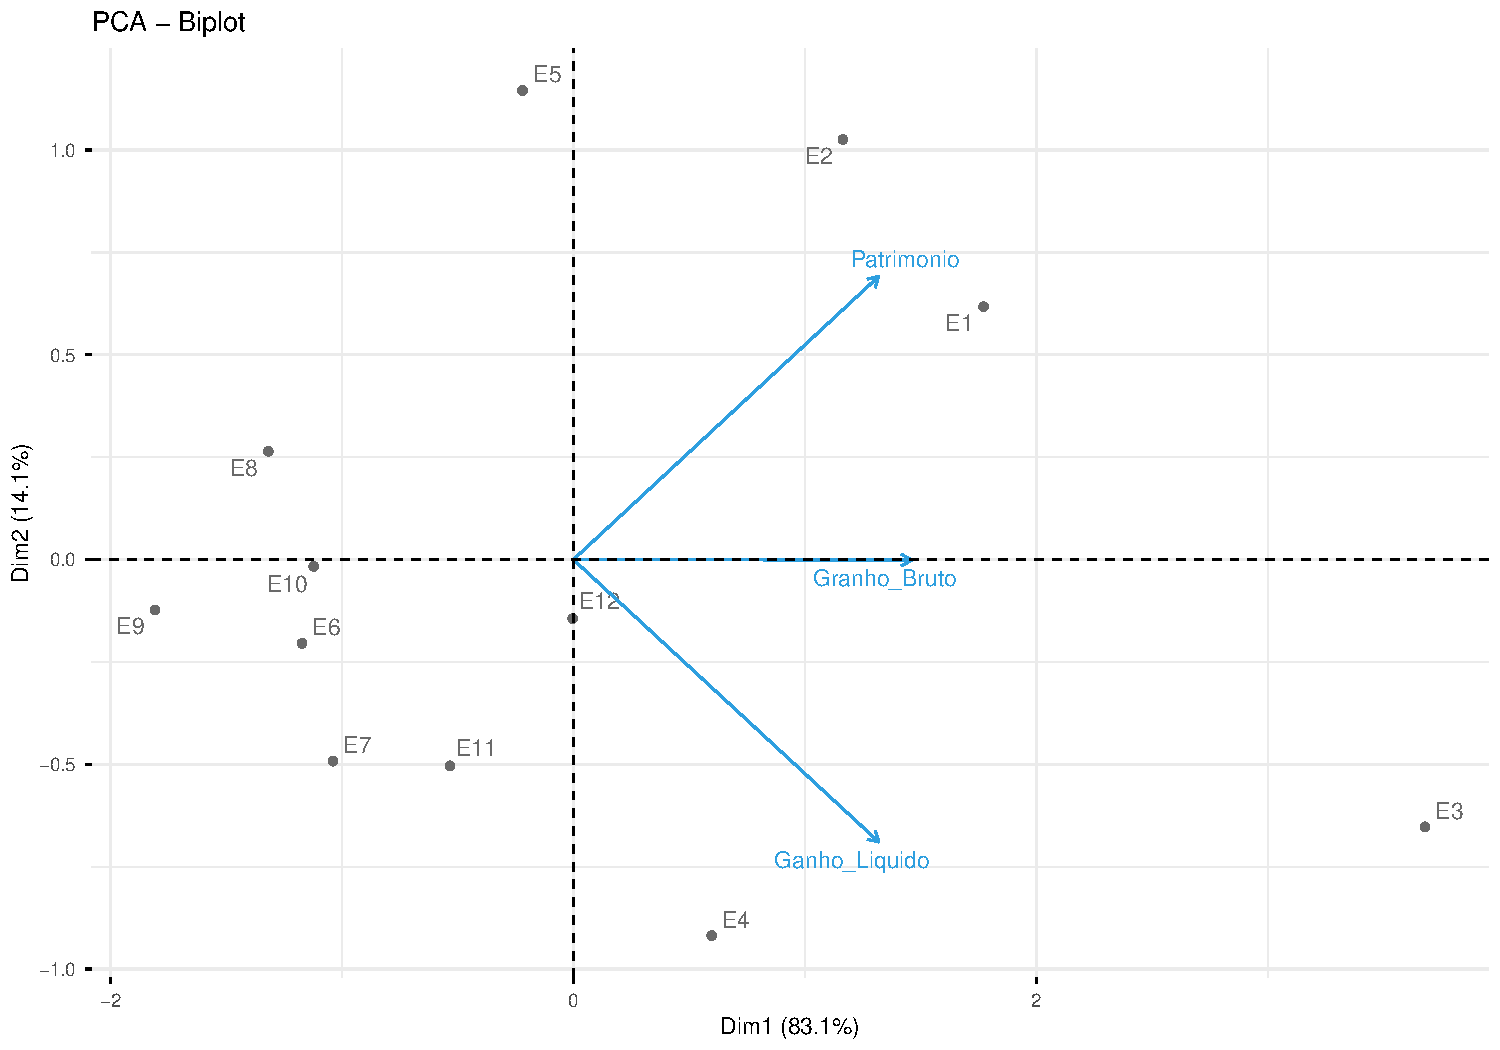
\includegraphics[width=0.7\linewidth,height=\textheight,keepaspectratio]{comp_princ_files/figure-beamer/unnamed-chunk-15-1.pdf}
\end{center}
\end{frame}

\begin{frame}{Voltando ao Exemplo}
\phantomsection\label{voltando-ao-exemplo-11}
\textbf{Interpretação do biplot}

\begin{itemize}
\tightlist
\item
  As setas indicam em que direção a variável aumenta. os indivíduos que
  estão posicionados no sentido da seta são os que têm valores maiores
  naquela variável.
\end{itemize}

\pause

\begin{itemize}
\tightlist
\item
  \textbf{Ângulo entre a seta (variável) e o eixo PC1:} O cosseno do
  ângulo entre a variável e a PC é exatamente o \textbf{loading}.
\end{itemize}

\[\cos(\theta_j, PC_i) = \text{loading}_{X_j, PC_i}\]
\end{frame}

\begin{frame}{Voltando ao Exemplo}
\phantomsection\label{voltando-ao-exemplo-12}
então:

\begin{itemize}
\tightlist
\item
  se a seta está quase colada no eixo \(PC_i\)

  \begin{itemize}
  \tightlist
  \item
    loading próximo de +1 → variável altamente alinhada com a componente
  \item
    é variável que define o componente principal
  \end{itemize}
\item
  se a seta faz um ângulo grande (perto de 90°) com \(PC_i\)

  \begin{itemize}
  \tightlist
  \item
    loading \(\approx 0\) → essa variável não contribui para a
    componente
  \end{itemize}
\item
  se a seta aponta para o lado oposto da \(PC_i\) (180°)

  \begin{itemize}
  \tightlist
  \item
    loading \(\approx -1\) → variável altamente alinhada negativamente
  \end{itemize}
\end{itemize}
\end{frame}

\begin{frame}{Voltando ao Exemplo}
\phantomsection\label{voltando-ao-exemplo-13}
\begin{itemize}
\tightlist
\item
  \textbf{Observação:} Quando a PCA é feita na \textbf{matriz de
  correlações}, os loadings são exatamente as correlações entre as
  variáveis originais e as componentes principais. Quando usamos
  \textbf{matriz de covariâncias}, os loadings refletem contribuição em
  variância e o cosseno do ângulo não corresponde numericamente à
  correlação.
\end{itemize}
\end{frame}

\begin{frame}{Voltando ao Exemplo}
\phantomsection\label{voltando-ao-exemplo-14}
\begin{itemize}
\tightlist
\item
  \textbf{PC1 (Dim1 = 83.1\%):} Praticamente toda a informação relevante
  está aqui.
\end{itemize}

\begin{quote}
PC1 representa um eixo geral de nível financeiro / escala econômica.
Quanto maior Patrimônio / Ganho Bruto / Ganho Líquido → mais à direita o
indivíduo aparece.
\end{quote}

\begin{itemize}
\tightlist
\item
  Todas variáveis apontam para a direita, e com ângulos semelhantes →
  altíssima correlação entre elas
\end{itemize}
\end{frame}

\begin{frame}{Voltando ao Exemplo}
\phantomsection\label{voltando-ao-exemplo-15}
\begin{itemize}
\item
  Quem está mais pra direita (E1, E2, E3) → são aqueles com valores
  altos nessas variáveis
\item
  Quem está mais pra esquerda (E8, E9, E10\ldots) → são os com valores
  baixos
\item
  A empresa E12 posiciona-se muito próxima à origem do plano principal,
  indicando um perfil mediano em todas as variáveis financeiras
  consideradas.

  \begin{itemize}
  \tightlist
  \item
    Ela não apresenta características extremas nem para valores altos,
    nem para valores baixos, sendo portanto uma empresa altamente
    representativa do centro da distribuição.
  \end{itemize}
\end{itemize}

\pause

\begin{itemize}
\tightlist
\item
  \textbf{PC2 (Dim2 = 14.1\%):} quase não traz informação nova → setas
  não sobem muito, elas estão quase horizontais

  \begin{itemize}
  \tightlist
  \item
    não existe uma segunda dimensão ``conceitual'' forte
  \end{itemize}
\end{itemize}
\end{frame}

\begin{frame}[fragile]{Voltando a Exemplo}
\phantomsection\label{voltando-a-exemplo}
\begin{Shaded}
\begin{Highlighting}[]
\CommentTok{\# Contribuições das variáveis para a PC1}
\FunctionTok{fviz\_contrib}\NormalTok{(acp\_R, }\AttributeTok{choice =} \StringTok{"var"}\NormalTok{, }\AttributeTok{axes =} \DecValTok{1}\NormalTok{)}
\end{Highlighting}
\end{Shaded}

\begin{center}
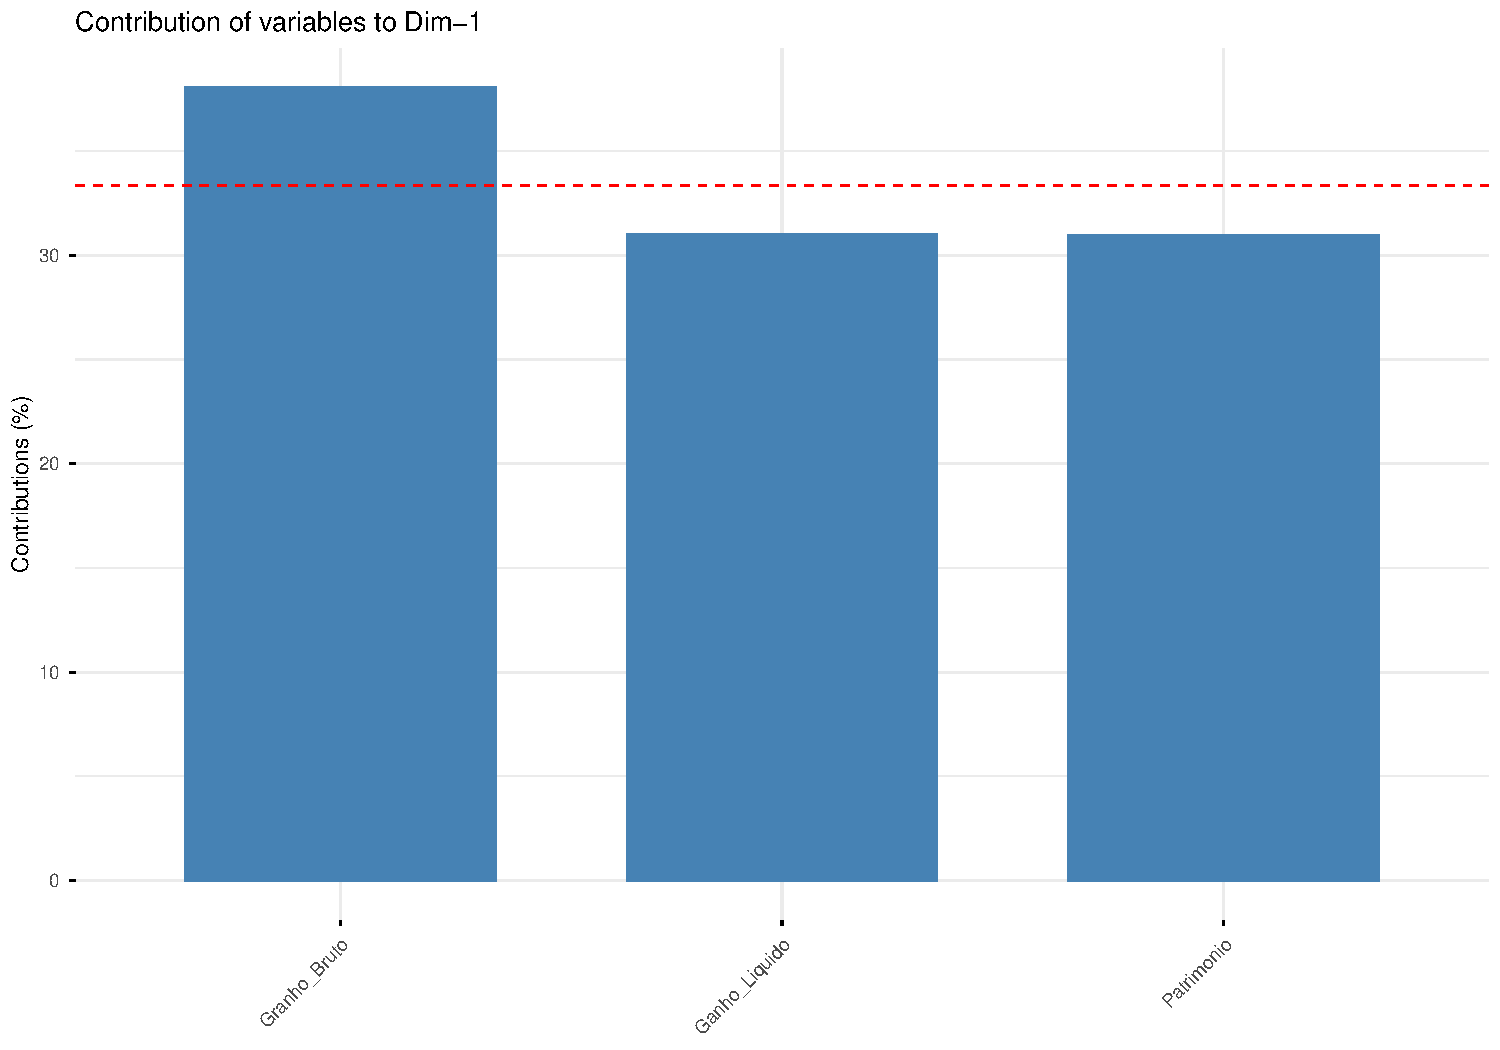
\includegraphics[width=0.7\linewidth,height=\textheight,keepaspectratio]{comp_princ_files/figure-beamer/unnamed-chunk-16-1.pdf}
\end{center}
\end{frame}

\begin{frame}{Voltando ao Exemplo}
\phantomsection\label{voltando-ao-exemplo-16}
\begin{itemize}
\tightlist
\item
  Esse gráfico mostra o quanto cada variável explica/contribui para a
  formação do primeiro componente principal.

  \begin{itemize}
  \tightlist
  \item
    Ganho Bruto contribuiu um pouco mais
  \item
    Ganho Liquido e Patrimonio contribuem praticamente igual e muito
    próximo
  \end{itemize}
\end{itemize}

\pause

\begin{itemize}
\tightlist
\item
  A linha vermelha tracejada é a contribuição média esperada (se todas
  contribuíssem igual).

  \begin{itemize}
  \tightlist
  \item
    Como temos 3 variáveis → contribuição média =
    \(100\%/3 \approx 33.33\%\)
  \end{itemize}
\end{itemize}
\end{frame}

\begin{frame}[fragile]{Voltando ao Exemplo}
\phantomsection\label{voltando-ao-exemplo-17}
\begin{Shaded}
\begin{Highlighting}[]
\FunctionTok{fviz\_contrib}\NormalTok{(acp\_R, }\AttributeTok{choice =} \StringTok{"ind"}\NormalTok{, }\AttributeTok{axes =} \DecValTok{1}\SpecialCharTok{:}\DecValTok{2}\NormalTok{)}
\end{Highlighting}
\end{Shaded}

\begin{center}
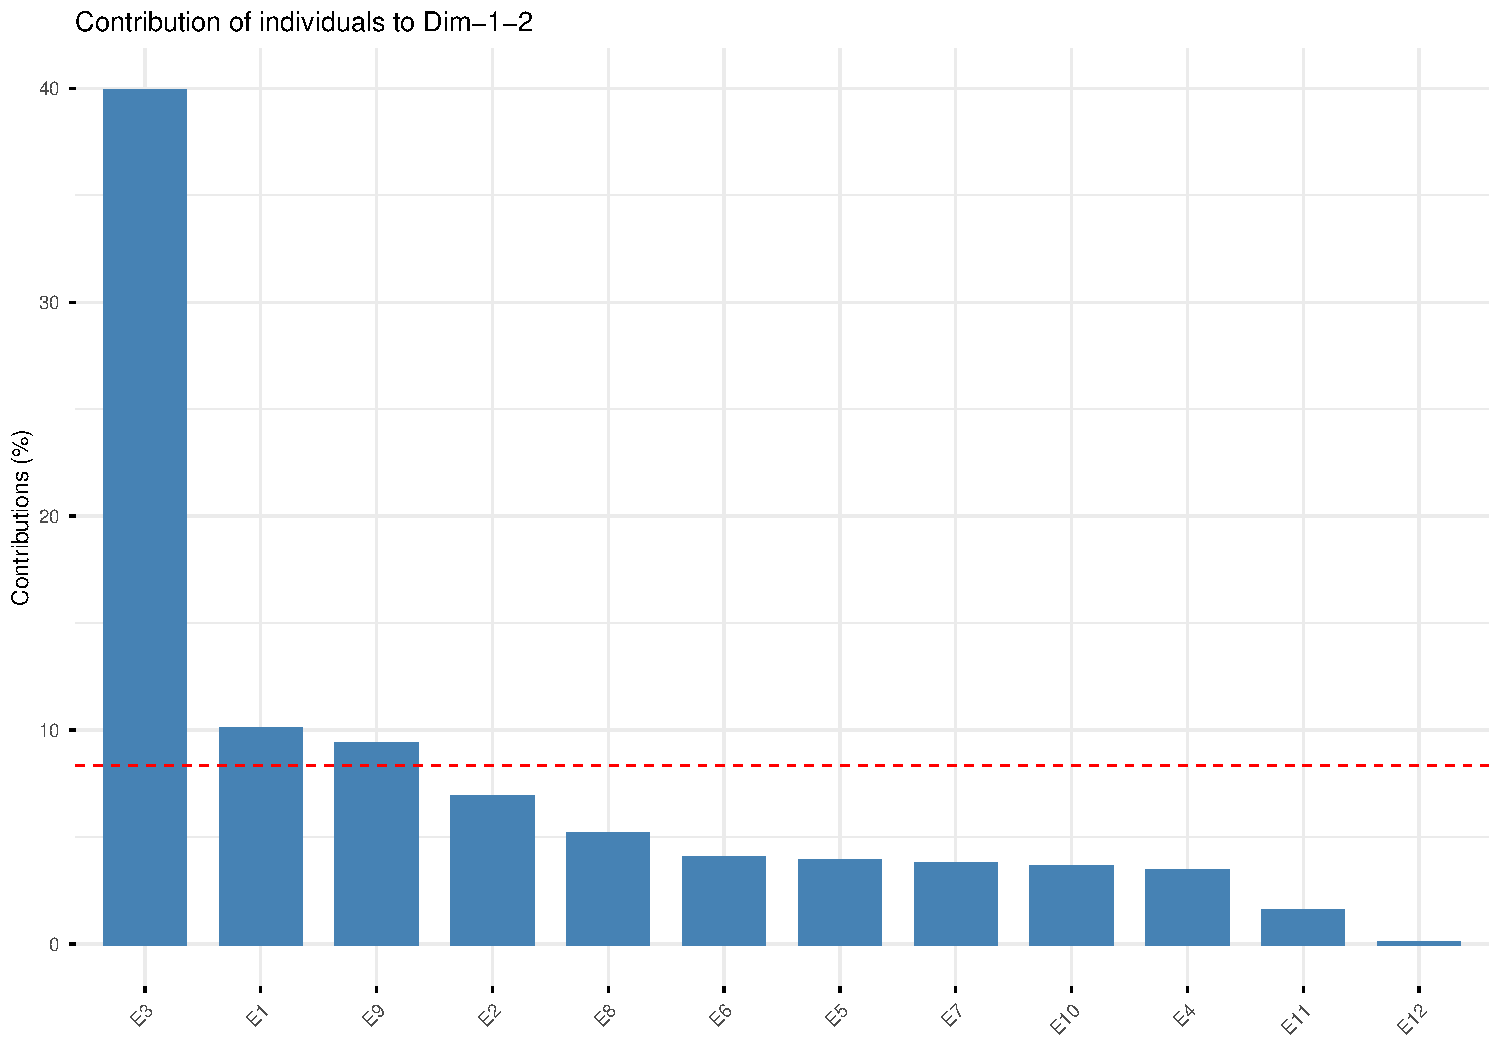
\includegraphics[width=0.7\linewidth,height=\textheight,keepaspectratio]{comp_princ_files/figure-beamer/unnamed-chunk-17-1.pdf}
\end{center}
\end{frame}

\begin{frame}{Voltando ao Exemplo}
\phantomsection\label{voltando-ao-exemplo-18}
\begin{itemize}
\tightlist
\item
  Esse gráfico mostra quais indivíduos contribuem mais para definir o
  plano principal da PC, isto é, quais observações estão orientando a
  direção das componentes principais.
\end{itemize}

\pause

\begin{itemize}
\tightlist
\item
  A empresa E3 é a maior influenciadora da PCA: sua contribuição para o
  plano principal é muito superior à média (linha vermelha), indicando
  que ela é um caso extremo na direção da primeira componente. Esse
  ponto está orientando de forma dominante a estrutura da análise.
\end{itemize}
\end{frame}




\end{document}
